%!TEX TS-program = xelatex

% kudos to
% Author: Amet Umerov (admin@amet13.name)
% https://github.com/Amet13/master-thesis

\documentclass[xetex,a4paper,14pt]{extarticle} % 14й шрифт
%%% Преамбула %%%

\usepackage{fontspec} % XeTeX
\usepackage{xunicode} % Unicode для XeTeX
\usepackage{xltxtra}  % Верхние и нижние индексы
\usepackage{pdfpages} % Вставка PDF

\usepackage{listings} % Оформление исходного кода
\lstset{
    basicstyle=\small\ttfamily, % Размер и тип шрифта
    breaklines=true,            % Перенос строк
    tabsize=2,                  % Размер табуляции
    frame=single,               % Рамка
    literate={--}{{-{}-}}2,     % Корректно отображать двойной дефис
    literate={---}{{-{}-{}-}}3  % Корректно отображать тройной дефис
}

% Шрифты, xelatex
\defaultfontfeatures{Ligatures=TeX}
\setmainfont{Times New Roman} % Нормоконтроллеры хотят именно его
\newfontfamily\cyrillicfont{Times New Roman}
% \setsansfont{Liberation Sans} % Тут я его не использую, но если пригодится
\setmonofont{FreeMono} % Моноширинный шрифт для оформления кода

% Формулы
\usepackage{mathtools,unicode-math} % Не совместим с amsmath
\setmathfont{XITS Math}             % Шрифт для формул: https://github.com/khaledhosny/xits-math
\numberwithin{equation}{section}    % Формула вида секция.номер

% Русский язык
\usepackage{polyglossia}
\setdefaultlanguage{russian}

% Абзацы и списки
\usepackage{enumerate}   % Тонкая настройка списков
\usepackage{indentfirst} % Красная строка после заголовка
\usepackage{float}       % Расширенное управление плавающими объектами
\usepackage{multirow}    % Сложные таблицы

% Пути к каталогам с изображениями
\usepackage{graphicx} % Вставка картинок и дополнений
\graphicspath{{images/}}

% Формат подрисуночных записей
\usepackage{chngcntr}

% Сбрасываем счетчик таблиц и рисунков в каждой новой главе
\counterwithin{figure}{section}
\counterwithin{table}{section}

% Гиперссылки
\usepackage{hyperref}
\hypersetup{
    colorlinks, urlcolor={black}, % Все ссылки черного цвета, кликабельные
    linkcolor={black}, citecolor={black}, filecolor={black},
    pdfauthor={Orlovsky Maxim},
    pdftitle={No title}
}

% Оформление библиографии и подрисуночных записей через точку
\makeatletter
\renewcommand*{\@biblabel}[1]{\hfill#1.}
\renewcommand*\l@section{\@dottedtocline{1}{1em}{1em}}
\renewcommand{\thefigure}{\thesection.\arabic{figure}} % Формат рисунка секция.номер
\renewcommand{\thetable}{\thesection.\arabic{table}}   % Формат таблицы секция.номер
\def\redeflsection{\def\l@section{\@dottedtocline{1}{0em}{10em}}}
\makeatother

\renewcommand{\baselinestretch}{1.4} % Полуторный межстрочный интервал
\parindent 1.27cm % Абзацный отступ

\sloppy             % Избавляемся от переполнений
\hyphenpenalty=1000 % Частота переносов
\clubpenalty=10000  % Запрещаем разрыв страницы после первой строки абзаца
\widowpenalty=10000 % Запрещаем разрыв страницы после последней строки абзаца

% Отступы у страниц
\usepackage{geometry}
\geometry{left=3cm}
\geometry{right=1cm}
\geometry{top=2cm}
\geometry{bottom=2cm}

% Списки
\usepackage{enumitem}
\setlist[enumerate,itemize]{leftmargin=12.7mm} % Отступы в списках

\makeatletter
    \AddEnumerateCounter{\asbuk}{\@asbuk}{м)}
\makeatother
\setlist{nolistsep}                           % Нет отступов между пунктами списка
\renewcommand{\labelitemi}{--}                % Маркер списка --
\renewcommand{\labelenumi}{\asbuk{enumi})}    % Список второго уровня
\renewcommand{\labelenumii}{\arabic{enumii})} % Список третьего уровня

% Содержание
\usepackage{tocloft}
\renewcommand{\cfttoctitlefont}{\hspace{0.38\textwidth}\MakeTextUppercase} % СОДЕРЖАНИЕ
\renewcommand{\cftsecfont}{\hspace{0pt}}            % Имена секций в содержании не жирным шрифтом
\renewcommand\cftsecleader{\cftdotfill{\cftdotsep}} % Точки для секций в содержании
\renewcommand\cftsecpagefont{\mdseries}             % Номера страниц не жирные
\setcounter{tocdepth}{3}                            % Глубина оглавления, до subsubsection

% Список иллюстративного материала
\renewcommand{\cftloftitlefont}{\hspace{0.17\textwidth}\MakeTextUppercase}
\renewcommand{\cftfigfont}{Рисунок }
\addto\captionsrussian{\renewcommand\listfigurename{Список иллюстративного материала}}

% Список табличного материала
\renewcommand{\cftlottitlefont}{\hspace{0.2\textwidth}\MakeTextUppercase}
\renewcommand{\cfttabfont}{Таблица }
\addto\captionsrussian{\renewcommand\listtablename{Список табличного материала}}

% Нумерация страниц посередине сверху
\usepackage{fancyhdr}
\pagestyle{fancy}
\fancyhf{}
\cfoot{\textrm{\thepage}}
\fancyheadoffset{0mm}
\fancyfootoffset{0mm}
\setlength{\headheight}{17pt}
\renewcommand{\headrulewidth}{0pt}
\renewcommand{\footrulewidth}{0pt}
\fancypagestyle{plain}{
    \fancyhf{}
    \cfoot{\textrm{\thepage}}
}

% Формат подрисуночных надписей
\RequirePackage{caption}
\DeclareCaptionLabelSeparator{defffis}{ -- } % Разделитель
\captionsetup[figure]{justification=centering, labelsep=defffis, format=plain} % Подпись рисунка по центру
\captionsetup[table]{justification=raggedright, labelsep=defffis, format=plain, singlelinecheck=false} % Подпись таблицы слева
\addto\captionsrussian{\renewcommand{\figurename}{Рисунок}} % Имя фигуры

% Пользовательские функции
\newcommand{\addimg}[4]{ % Добавление одного рисунка
    \begin{figure}
        \centering
        \includegraphics[width=#2\linewidth]{#1}
        \caption{#3} \label{#4}
    \end{figure}
}
\newcommand{\addimghere}[4]{ % Добавить рисунок непосредственно в это место
    \begin{figure}[H]
        \centering
        \includegraphics[width=#2\linewidth]{#1}
        \caption{#3} \label{#4}
    \end{figure}
}
\newcommand{\addtwoimghere}[5]{ % Вставка двух рисунков
    \begin{figure}[H]
        \centering
        \includegraphics[width=#2\linewidth]{#1}
        \hfill
        \includegraphics[width=#3\linewidth]{#2}
        \caption{#4} \label{#5}
    \end{figure}
}

% Заголовки секций в оглавлении в верхнем регистре
\usepackage{textcase}
\makeatletter
\let\oldcontentsline\contentsline
\def\contentsline#1#2{
    \expandafter\ifx\csname l@#1\endcsname\l@section
        \expandafter\@firstoftwo
    \else
        \expandafter\@secondoftwo
    \fi
    {\oldcontentsline{#1}{\MakeTextUppercase{#2}}}
    {\oldcontentsline{#1}{#2}}
}
\makeatother

% Оформление заголовков
\usepackage[compact,explicit]{titlesec}
\titleformat{\section}{}{}{12.5mm}{\centering{\thesection\quad\MakeTextUppercase{#1}}\vspace{1.5em}}
\titleformat{\subsection}[block]{\vspace{1em}}{}{12.5mm}{\thesubsection\quad#1\vspace{1em}}
\titleformat{\subsubsection}[block]{\vspace{1em}\normalsize}{}{12.5mm}{\thesubsubsection\quad#1\vspace{1em}}
\titleformat{\paragraph}[block]{\normalsize}{}{12.5mm}{\MakeTextUppercase{#1}}

% Секции без номеров (введение, заключение...), вместо section*{}
\newcommand{\anonsection}[1]{
    \phantomsection % Корректный переход по ссылкам в содержании
    \paragraph{\centerline{{#1}}\vspace{1em}}
    \addcontentsline{toc}{section}{#1}
}

% Секция для аннотации (она не включается в содержание)
\newcommand{\annotation}[1]{
    \paragraph{\centerline{{#1}}\vspace{1em}}
}

% Секция для списка иллюстративного материала
\newcommand{\lof}{
    \phantomsection
    \listoffigures
    \addcontentsline{toc}{section}{\listfigurename}
}

% Секция для списка табличного материала
\newcommand{\lot}{
    \phantomsection
    \listoftables
    \addcontentsline{toc}{section}{\listtablename}
}

% Секции для приложений
\newcommand{\appsection}[1]{
    \phantomsection
    \paragraph{\centerline{{#1}}}
    \addcontentsline{toc}{section}{{#1}}
}

% Библиография: отступы и межстрочный интервал
\makeatletter
\renewenvironment{thebibliography}[1]
    {\section*{\refname}
        \list{\@biblabel{\@arabic\c@enumiv}}
           {\settowidth\labelwidth{\@biblabel{#1}}
            \leftmargin\labelsep
            \itemindent 16.7mm
            \@openbib@code
            \usecounter{enumiv}
            \let\p@enumiv\@empty
            \renewcommand\theenumiv{\@arabic\c@enumiv}
        }
        \setlength{\itemsep}{0pt}
    }
\makeatother

\usepackage{lastpage} % Подсчет количества страниц
\setcounter{page}{3}  % Начало нумерации страниц % Подключаем преамбулу

%%% Начало документа
\begin{document}

% 1 страница
% \includepdf{extra/pz} % Пояснительная записка

% 2 страница (не нумеруется, но учитывается)
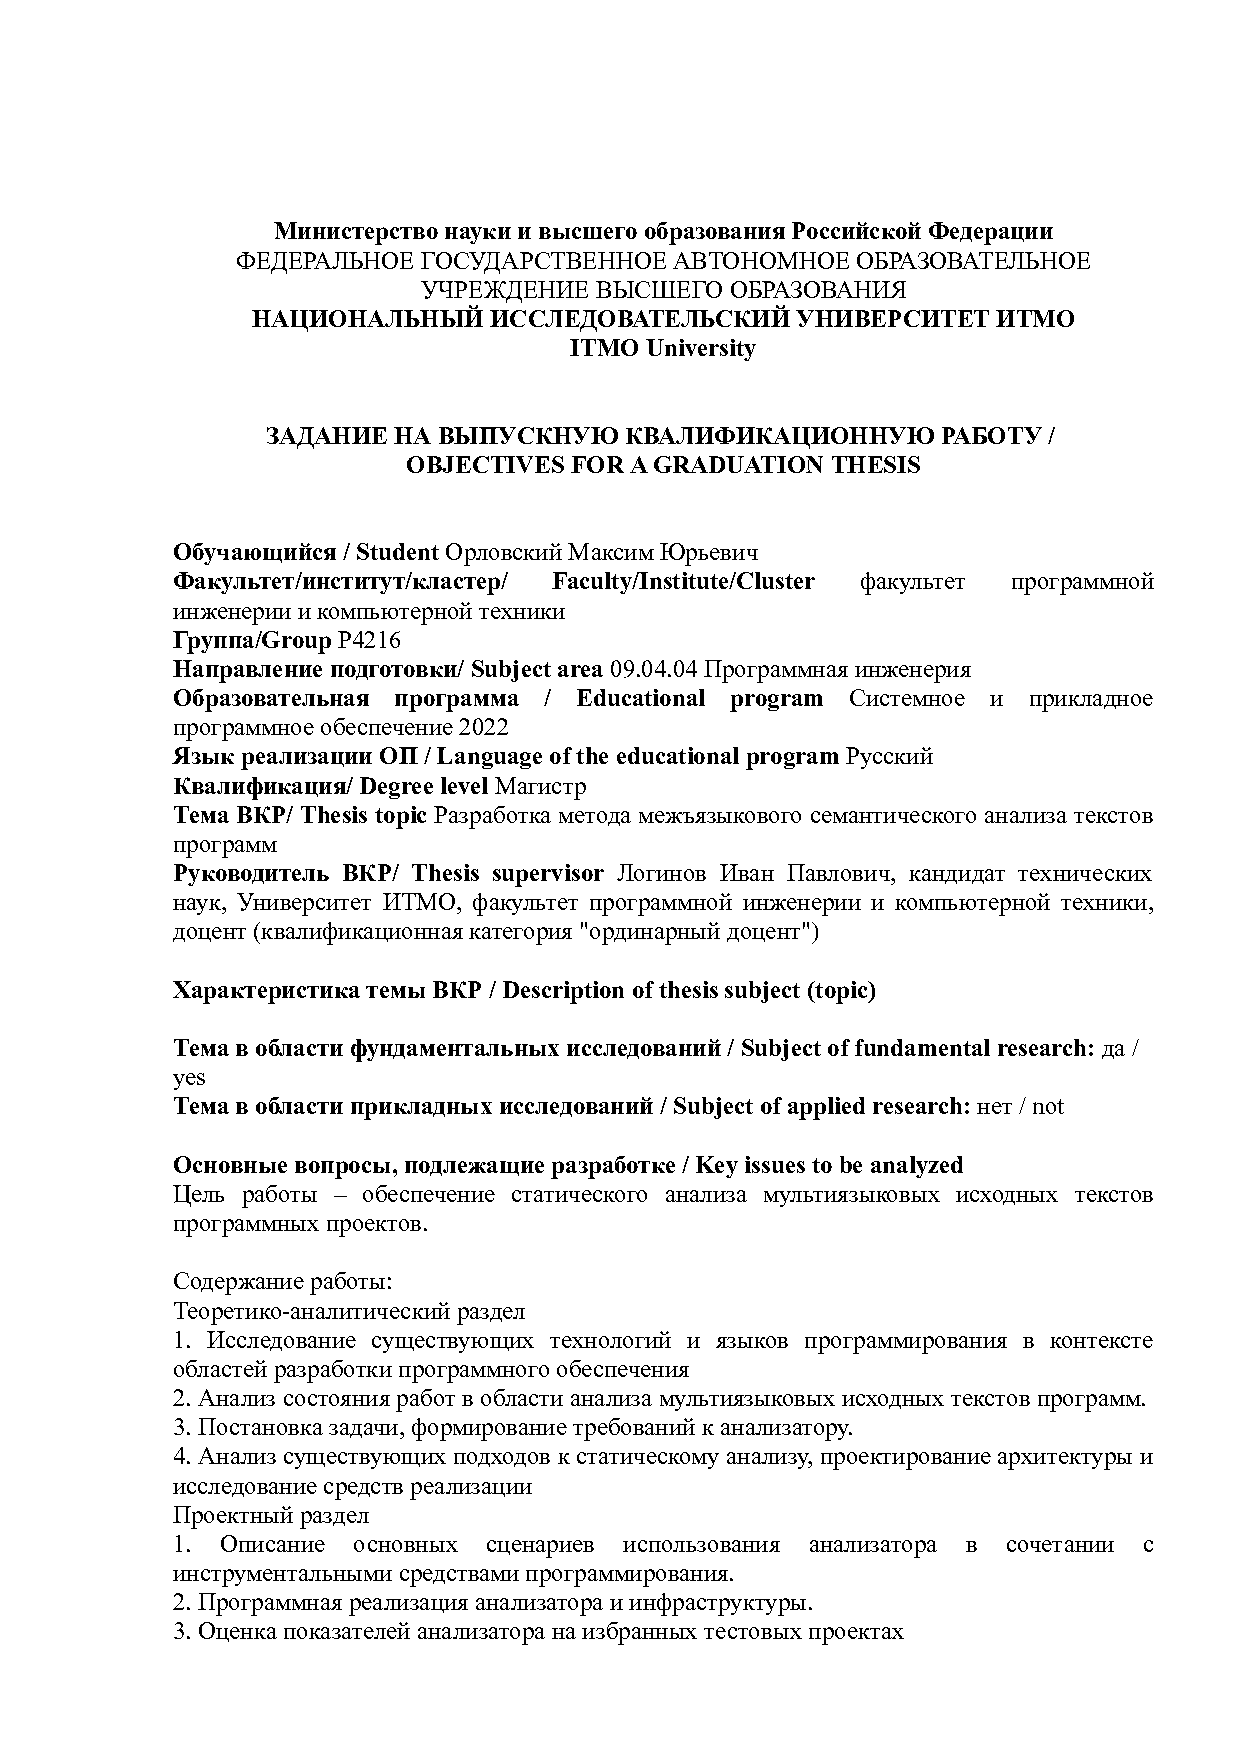
\includepdf[pages={1,2}]{extra/tz} % Задание на ВКР печатается на одном листе с двух сторон

% Помимо ПЗ и задания, в ВКР также вкладываются:
% * отзыв руководителя (otzyv.pdf), на 1 странице с двух сторон
% * рецензия (review.pdf), на 1 странице с двух сторон
% * отчет по антиплагиату (antiplagiat.pdf)

% 3 страница
\annotation{Аннотация}

Тема выпускной квалификационной работы магистра --- <<Исследование процессов обеспечения безопасности облачных сред>>.

Ключевые слова: безопасность, виртуализация, защита информации, облачная инфраструктура, облачные вычисления, провайдер, стандартизация, уязвимости.

Актуальность темы.
В настоящее время наблюдается стремительное развитие облачных технологий, однако для эффективной работы облачной инфраструктуры требуется ее эффективная структура и организация.
Зачастую небольшая команда, проектирующая облачную инфраструктуру не всегда может полностью учесть все аспекты безопасности, так как нет единого документа, стандартизующего механизмы обеспечения безопасности в облачной среде.
Особенно остро вопрос безопасности встал в последнее время, в связи с обнаружением большого количества критических уязвимостей в программном обеспечении и протоколах, используемых поставщиками облачных услуг.

Целью проводимых исследований является повышение эффективности процессов обеспечения информационной безопасности облачных сред.
Для достижения поставленной цели необходимо разработать структуру системы обеспечения информационной безопасности  заданной облачной среды, провести внедрение и экспериментальные исследования.

Выпускная квалификационная работа магистра изложена на \pageref{LastPage} листах, включает 16 таблиц, 12 рисунков, 1 приложение, 27 литературных источников.

\clearpage
 % Аннотация

\tableofcontents % Содержание 
\clearpage

\anonsection{Введение}

Облачные услуги --- это способ предоставления, потребления и управления технологией.
Данный тип услуг выводит гибкость и эффективность на новый уровень, путем эволюции способов управления, таких как непрерывность, безопасность, резервирование и самообслуживание, которые соединяют физическую и виртуальную среду.

Для эффективной работы облачной инфраструктуры требуется эффективная структура и организация.
Небольшая команда из специалистов и бизнес-пользователей может создать обоснованный план и организовать свою работу в подобной инфраструктуре.
Данная выделенная группа может намного эффективнее построить и управлять нестандартной облачной инфраструктурой, чем если компании будут просто продолжать добавлять дополнительные сервера и сервисы для поддержки центра обработки данных (\hyperlink{dc}{ЦОД}).

Развитие информационного мира движется в сторону повсеместного распространения облачных вычислений, их технологий и сервисов.
Очевидные преимущества данного подхода \cite{telecom-world}:
\begin{itemize}
  \item снижение затрат --- отсутствие необходимости покупки собственного оборудования, программного обеспечения (\hyperlink{soft}{ПО}), работы системного инженера;
  \item удаленный доступ --- возможность доступа к данным облака из любой точки мира, где есть доступ в глобальную сеть Интернет;
  \item отказоустойчивость и масштабируемость --- изменение необходимых ресурсов в зависимости от потребностей проекта, техническое обслуживание оборудования лежит на плечах облачного провайдера.
\end{itemize}

В связи с этим можно сделать вывод, что основные недостатки облачных вычислений сводятся к информационной безопасности.
Такого мнения придерживаются многие крупные информационные компании, что в некоторой степени препятствует более стремительному развитию рынка облачных сервисов.

\clearpage
        % Введение
\section{Исследование существующих технологий и языков программирования в контексте
областей разработки программного обеспечения}

\subsection{Современная индустрия разработки программного обеспечения}

Современные программные проекты, в отличие от многих программных проектов прошлого,
гораздо чаще состоят из набора разных (порой разительно) технологических
решений, предназначенных для решения определенного круга задач. Согласно \cite{empirical-analysis},
в одном программном проекте в среднем задействовано 5 языков программирования, один из
которых является <<основным>>, о остальные -- специализированными языками предметной области (\hyperlink{DSL}{DSL}).
В заключении статьи авторы признают популярность мультиязыковых программных проектов
и оценивают важность наличия соответствующих инструментальных средств для работы с
такого рода проектами.

Также, нередко использование нескольких языков и в индустрии разработки. Так, авторы \cite{professional-developers}
провели исследование популярности мультиязыковых проектов
в результате опроса 139 профессиональных разработчиков из разных сфер. 
Результаты опроса показали, что опрашиваемые имели дело с 7 различными языками, в среднем.
При этом, в работу было вовлечено в среднем 3 пары связанных языков в контексте одного проекта.
Более 90\% опрашиваемых также сообщали о проблемах согласованности между языками,
встречаемых при разработке в такой мультиязыковой среде. 

Таким образом, в современной разработке программного обеспечения нередко использование
нескольких языков вне зависимости от объемов проекта или вовлекаемой предметной области.
Ситуация становится сложнее со временем, так как создание новых технологий разработки
часто влечет за собой формирование определенной нотации или языка для управления или конфигурации.
Например, это может касаться таких повсеместных технологий как \hyperlink{СУБД}{СУБД}, система сборки,
сервер приложений или скрипты развертывания.

Для наглядности, можно привести следующие языки, нередко фигурирующие в составе современных программных проектов:
\begin{itemize}    
    \item язык разметки HTML в составе проекта, использующего ASP фреймворк,
    \item язык скриптов командной строки в составе проекта, использующего язык C,
    \item язык запросов SQL в составе проекта, использующего Python и фреймворк Flask,
    \item язык препроцессора в составе файла исходного кода, реализованного на C++.
\end{itemize}
Заключительный пункт списка примеров приведен для того, чтобы показать характер
связи различных технологий —- разным языкам необязательно даже находится в раздельных
файлах или модулях, нередки случаи полноценного переплетения различных синтаксисов и
семантик.

\subsection{Актуальность мультиязыкового статического анализа}

Итак, мультиязыковые программные проекты нередки. Следовательно, имеет смысл использования
различных техник работы с исходным кодом таких проектов, поддерживающих процесс разработки.
Одной из таких техник, обеспечивающей разные сценарии использования, является статический анализ
исходного кода. 

Стоит уточнить что имеется под определением <<статический анализ кода>>. Статический
анализ это прежде всего набор различных техник по извлечению информации о программе без
явного её запуска \cite{static-program-analysis}. Таким образом, статический анализ может
быть полезен в сценариях, которые не предполагают явного запуска программы -- в сущности во
всех сценариях процесса разработки ПО исключая этапы тестирования и запуска.

Возможные сценарии использования статического анализа кода включают (но не ограничиваются):
\begin{itemize}
    \item оптимизацию программ,
    \item выявление потенциальных уязвимостей,
    \item доказательство сохранения определенных инвариантов,
    \item сбор определенной статистики,
    \item выявление <<пахнущих>> фрагментов кода,
    \item помощь разработчику во время кодирования,
    \item автоматический рефакторинг кода.
\end{itemize}

Так как сценарии использования статического анализа настолько разнообразны, в рамках данной работы
решено было сосредоточится на аспектах разработки, которые помогают в процессе кодирования и поддержки проекта.
В качестве прикладной реализации таких аспектов выступают различные инструментальные средства.
К таким средствам, к примеру, относятся:
\begin{itemize}
    \item интегрированные средства разработки (\hyperlink{IDE}{IDE}),
    \item линтеры (собирательное название инструментов, первым из которых был <<Lint>> \cite{linter}),
    \item инструменты автоматического рефакторинга,
    \item инструменты сбора статистики,
    \item различные кодогенераторы и фреймворки \cite{qt-moc}\cite{react}.
\end{itemize}

Необходимость в таких средствах присутствует и она достаточно высока. Так, согласно
исследованию \cite{aid-developers}, использование средств поддержки разработчика
(в данной работе это механизмы анализа и навигации по межъязыковым связям) позволяет
улучшить как скорость разработки ПО, так и уменьшить количество совершаемых ошибок. Стоит заметить,
что несмотря на количество времени, прошедшее с момента проведения исследования, 
принципы разработки ПО в данной предметной области (веб-разработка) не изменились и большинство
программных проектов веб-приложений состоят как минимум из двух языков. 
Обычно это разделение проводится по принципу фронтенд и бекенд.

Согласно обзорной статье об исследовании межъязыковых связей \cite{pragmatic-evidence}, современные средства межъязыкового
и мультиязыкового анализа остаются всё еще плохо развитыми. Особенно это касается отношения корректности
таких средств. Более того, большая их часть часто является частным решением, ориентированным на определенную
предметную область или технологию, что снижает универсальность таких средств и усложняет их интеграцию.

Так как статья содержит большую выборку литературы по обнаружению и анализу межъязыковых связей, авторам удается
установить широкую область применения межъязыкового анализа. В эту область входят такие дисциплины разработки ПО:
\begin{itemize}
    \item семантическое понимание программ,
    \item представление знаний при сопровождении систем,
    \item рефакторинг,
    \item моделирование ПО,
    \item валидация и верификация систем,
    \item визуализация систем,
    \item сбор статистик и метрик.
\end{itemize}
Как видно из списка, большинство этих дисциплин значительно пересекаются со сценариями использования
статического анализа кода, что говорит о том что реализация такого анализа может быть очень актуальной
для обеспечения упрощения и удешевления большого количества этапов разработки ПО.

\subsection{Особенности мультиязыкового анализа} \label{ssec:num1}

Мультиязыковой анализ вовлекает множество особенностей существующих инструментов, так как косвенно или
непосредственно семантическая информация об этих инструментах должна быть вовлечена в процесс анализа.
Поэтому стоит рассмотреть особенности мультиязыкового анализа которые затрудняют разработку соответствующих
анализаторов и процесс анализа в целом.

\subsubsection{Сложности распознавания текста}

Так как вовлекаемые фрагменты кода написаны на разных языках, проблема анализа таких фрагментов
возникает уже на самом первом этапе -- этапе распознавания текста. Обычно процесс анализа
текста с определенной грамматикой не вызывает труда так как грамматика фиксирована и анализатор строится
стандартными средствами -- парсер генераторы, рекурсивный спуск и иные. 

Однако, в случае парсинга текста на нескольких языках возникает проблема так как создание универсальной
грамматики (для всех анализируемых языков) обычно либо сложно, либо невозможно. Таким образом остается
несколько способов распознавания текста:
\begin{enumerate}[label=\arabic*.]
    \item распознавание текстов по отдельности,
    \item использование смешанных парсеров (например с использованием островных грамматик \cite{island-grammars}),
    \item использование единого представления.
\end{enumerate}
Первый пункт является простым в реализации и работает в большинстве случаев, однако
возникают сложности при анализе единого фрагмента (например, файла), который вовлекает несколько
языков в анализ (к примеру CSS стили в заголовке страницы HTML). Второй пункт позволяет анализировать
смешанные грамматики в том числе, но сборка таких анализаторов довольно трудоемка и ограничена поддержкой
лишь определенного количества языков.

Таким образом, наиболее оптимальным является вариант распознавания при котором мультиязыковые фрагменты
изначально переводятся в единое представление (используя любой специфичный способ перевода, сохраняющий семантику), а
уже затем распознаются и анализируются. В некоторых случаях такой подход является наиболее удобным так как
интересующая область анализа может вовлекать только ту информацию, которая получается после преобразования в унифицированное
представление. В таком случае изначальное преобразование является семантически корректным этапом и позволяет
упросить анализатор.

\subsubsection{Анализ и кодогенерация}

Несмотря на то, что кодогенерация является сложностью которую приходится учитывать и при обычном
статическом анализе, в мультиязыковых проектах эта сложность выходит на новый уровень.
Это происходит в первую очередь потому что большое количество технологических решений, вовлекающих
разные языки используют разные подходы к кодогенерации и по разному её осуществляют.

Для понимания возможных проблем, рассмотрим следующий фрагмент кода на C++:
\begin{lstlisting}[numbers=left, language=C++]
// function.h
#include <stdio.h>
template <typename T>
T f(T a) {
#ifdef SOMEBAR
    return a * 2;
#else
    return a + 2;
#endif
}

// main.cpp
#include "function.h"
int main()
{
#ifdef SOMEFOO
    printf("%f", f<float>(10));
#else
    printf("%d", f<int>(5));
#endif
    return 0;
}
\end{lstlisting}

Представим что есть два файла, <<function.h>> и <<main.cpp>>. Фрагменты, соответствующие файлам, помечены
комментариями. При статическом анализе такого кода для определения того, какая версия функции в итоге будет
сгенерирована при компиляции необходимо сделать следующее:
\begin{enumerate}[label=\arabic*.]
    \item узнать какие значения принимают переменные среды при компиляции этих файлов,
    \item для каждого из таких значений сгенерировать возможную конфигурацию кода,
    \item проанализировать каждую конфигурацию и объединить результаты анализа.
\end{enumerate}
В отношении данного примера, возможных конфигураций будет четыре. В общем случае количество конфигураций
можно определить как мощность декартового произведения множеств значений вовлеченных переменных.
Нетрудно представить, что такое количество может быть достаточно большим, например при количестве переменных
равном 10 с учетом того что эти переменные принимают только 2 значения, количество конфигураций равно 1024.

Еще одной особенностью кодогенерации является частое вовлечение сторонних инструментов. В отличие от
примера приведенного выше, многие фреймворки различных технологических стеков полагаются на кодогенерацию во время
сборки проекта. Обычно эта кодогенерация вовлекает генерацию на уровне файлов. В данном случае статический анализ
не сможет обеспечить анализ сгенерированных файлов без использования одного из двух подходов:
\begin{itemize}
    \item запуск сборки и генерации во временной директории с последующей очисткой,
    \item абстрактная интерпретация команд генератора.
\end{itemize}

Первый подход может вызвать большие сложности если генерация имеет в зависимостях какое-либо
недоступное на момент анализа окружение. Примером может быть генерация файлов-прослоек для проекта,
который должен быть использован на конкретном встроенном устройстве. До момента размещения проекта
в специализированном окружении, нет информации о том какие прослойки необходимо генерировать.
Такое часто происходит при разработке встроенных систем по разным причинам: количество конфигураций
устройств, упрощение процесса разработки, недоступность устройств и т.д.

Второй подход является более сложным в реализации, так как различные кодогенераторы и фреймворки редко
имеют исчерпывающую документацию по особенностям кодогенерации, поэтому кодирование такой информации
часто будет неполным. Более того, особенности кодогенерации могут быть особенностью реализации
определенного инструмента, что может поменяться со временем. Поэтому, практическая реализация
таких анализаторов это сложный процесс, требующий большого количества времени и поддержки.

\subsubsection{Формирование выборки для анализа}

На первый взгляд формирование выборки кажется тривиальной проблемой. При моноязыковом анализе она
решается использованием сторонних инструментов, позволяющих получить набор файлов для анализа.
Такую информацию могут предоставлять системы сборки или развертывания, в крайнем случае достаточно
поиска в файловой системе определенного множества файлов.

Однако, при вовлечении нескольких языков в проект, получение соответствующих файлов путем простого
поиска может быть неадекватным решением по следующим причинам:
\begin{itemize}
    \item компоновка проекта из отдельных, несвязанных проектов,
    \item сборка проекта зависящая от условий в текущем окружении,
    \item специфика компоновки файлов в единый модуль зависит от конкретного языка и может отличаться.
\end{itemize}
Соответственно, для успешной практической интеграции анализатора, способного проводить мультиязыковой анализ
необходимо обеспечить также поддержку внешних инструментов, позволяющих правильно выбирать файлы для
анализа основываясь на конфигурации операционного окружения проекта. Таким образом, анализ проекта
первым этапом обязан обеспечивать анализ \textit{операционного окружения} проекта. Такая особенность
сильно усложняет анализатор и накладывает ограничения на технологии с которыми он может работать, так
как операционное окружение в общем случае включает состояние всего компьютера: файловая система, переменные
среды или реестр, подключение к сети и т.д. В данной работе проблема выборки файлов для анализа
не рассматривается в угоду упрощения анализатора и повышения его универсальности.

\subsubsection{Динамическая и неявная природа межъязыковых связей}

Многие семантически важные связи в реальных мультиязыковых проектах являются неявными. В большей части это применимо
к фреймворкам и системам сборки, так как порой семантическая информация распределена в разных местах проекта,
вовлекая при этом и системные зависимости \cite{professional-developers} \cite{external-dependencies}.

С точки зрения практической реализации, неявные связи являются усложняющим обстоятельством, но не
делающим анализ невозможным. К сожалению, то же нельзя сказать в отношении динамических связей. Под
динамическими связями понимаются связи, которые устанавливаются на определенном этапе исполнения кода.
Например, это может быть формирование строки коде JavaScript, которая потом может быть использована чтобы
получить определенные теги HTML страницы.

Несмотря на наличие динамических связей в определенных языках, значительное множество \hyperlink{GPL}{ языков общего назначения}
все же имеют статическую типизацию либо статическое время связывания идентификаторов. Это позволяет проводить
эффективный статический анализ таких языков. Однако, в случае гетерогенных проектов наличие динамической
связи гораздо более распространено. Это связано с различными причинами, основная из которых, возможно,
связана с разнообразием связываемых между собой технологий. Например, очень частой динамической (и часто
вполне явной) связью является зависимость фрагмента от состояния ФС. Это практически всегда встречается
в различных системах сборки -- скрипты сборки напрямую зависят от наличия некоторых файлов в системе и
при их отсутствии вынуждены прерывать исполнение сборки, порой после нескольких часов работы. Таким образом
тратятся как физические ресурсы, так и снижается продуктивность программиста, что может приводить к
ухудшению процесса разработки.

\subsubsection{Разнообразие парадигм программирования}

Как уже сказано в предыдущем подпункте, значительное множество \hyperlink{GPL}{GPL} являются статически типизированными
либо имеют статическое время связывания идентификаторов. Однако, это касается по большей части
императивных языков программирования. Примерами могут служить Java, C\#, C++, Golang и другие.
Многие \hyperlink{DSL}{DSL} однако, являются динамическими языками в том смысле, что они имеют позднее
связывание идентификаторов (обычно во время исполнения). Связано это в том числе с тем, что многие \hyperlink{DSL}{DSL}
имеют другую парадигму программирования, что также влияет на особенность их реализации. Примерами могут служить 
языки сборки, языки командной оболочки или языки выборки данных (например, запросов к \hyperlink{СУБД}{СУБД}).

Многие фреймворки <<программируются>> не напрямую, а через конфигурационные файлы. Примером может служить
повсеместный язык разметки XML, который иногда эксплуатируется как язык описания каких-либо выражений на
определенном \hyperlink{DSL}{DSL}. Ярким примером может служить система сборки Apache Ant, в ней узлы XML дерева
могут представлять обращения к переменным или даже целые выражения. Можно сказать, что любые конфигурационные
данные проекта могут представлять семантически важную информацию, так как использование конфигурационных
файлов в гетерогенных проектах повсеместно \cite{external-dependencies}.

Это приводит к тому, что некоторые вовлекаемые в анализ языки не являются языками программирования, но
всё же представляют семантическую ценность для анализа. Вследствие этого возникает проблема создания
такого анализа, который в том числе будет вовлекать такого рода фрагменты.

Подводя итоги подраздела \ref{ssec:num1}, можно сформировать следующие желаемые
особенности метода мультиязыкового анализа:
\begin{enumerate}[label=\arabic*.]
    \item анализ с использованием единого представления является более эффективным решением ввиду большей универсальности,
    \item желательна поддержка сценариев кодогенерации, либо возможность их реализации,
    \item необходимо вовлечение операционного окружения проекта для обеспечения корректности анализа,
    \item анализ должен быть универсальным для многих языков и парадигм программирования.
\end{enumerate}

\clearpage
\section{Анализ состояния работ в области анализа мультиязыковых исходных текстов программ}

% TODO: Использовать это как доказательство
https://arxiv.org/pdf/1906.00815.pdf

https://ieeexplore.ieee.org/abstract/document/7953501

\clearpage


% В т ч использовать \cite{pragmatic-evidence}
\section{Анализ существующих подходов к статическому анализу, проектирование архитектуры и
исследование средств реализации}

\subsubsection{Виды структур представления информации в статическом анализе}

Из подраздела \ref{ssec:2:results} становится ясно, что в отношении мультиязыкового анализа
основополагающим механизмом является наличие общей структуры представления информации, позволяющей отражать различные
сущности различных языков в единой форме. Выбор такой структуры может влиять на следующие
характеристики метода анализа:
\begin{itemize}
    \item разнообразие поддерживаемых языков,
    \item сложность разработки и поддержки анализаторов,
    \item корректность и полнота анализа,
    \item возможные сценарии использования.
\end{itemize}
В целом, выбор структуры влияет практически на все характеристики метода, поэтому стоит
исследовать существующие структуры представления информации о программном коде.

\hyperlink{AST}{AST} представляет собой репрезентацию программного кода в древовидном формате. В качестве узлов дерева выступают различные синтаксические конструкции, а в качестве ребер связи между ними. AST является
простой и универсальной структурой данных, позволяющей реализовывать множество анализов. Также,
носителем AST может быть любой структурный формат (например S-выражения), что упрощает его
построение, сериализацию и анализ. Однако, в контексте мультиязыкового анализа AST является
неудобным решением, в первую очередь потому что оно часто вовлекает языкоспецифичные конструкции.
К примеру, в некоторых языках отсутствует понятие <<оператор>> (англ statement), что различает
AST таких языков от императивных языков на фундаментальном уровне.

eCST \cite{eCST} является попыткой расширения концепции AST (а точнее \hyperlink{CST}{CST}) на большее
количество языков. Авторы достигают этого путем введения универсальных узлов, позволяющих
отражать общие семантические концепции (итерацию, выбор или переход). К сожалению, такой формат
представления информации всё еще неудобен так как языкоспецифичные узлы не могут быть конвертированы
в такие универсальные узлы и остаются в дереве в первозданном виде.

\hyperlink{CFG}{CFG} это граф, узлы которого представляют собой в общем случае операторы, а ребра
поток управления. Такой граф полезен в первую очередь для компиляторных трансформаций и оптимизаций,
так как позволяет моделировать исполнение программы и выстраивать на основе этого определенные инварианты.
Граф является основой для фреймворков монотонного анализа \cite{static-program-analysis} и активно
используется в различных инструментах. Несмотря на достоинства, как и в случае с AST такой граф
имеет зависимость от представляемого языка. Также, анализ потока управления сложен в контексте
мультиязыкового статического анализа и проще осуществим в рамках динамического анализа.

\hyperlink{CDG}{CDG} является формой представления информации о вызовах процедур друг другом в контексте
определенного фрагмента кода. Соотвественно, узлы такого графа обычно составляют идентификаторы
процедур, а ребра зависимость <<вызывает>>. Стоит сказать, что зависимость <<вызывает>> обычно является
направленной, поэтому граф имеет направление ребер. Такой граф является хорошим кандидатом на универсальное
представление в рамках мультиязыкового анализа, что уже было исследовано в \cite{MLSA}. Как было
сказано в подразделе \ref{ssec:mlsa}, основным недостатком графа зависимостей вызовов является
его ориентированность на процедуры -- исполняемые фрагменты кода. Это делает невозможным его применение
в рамках других языков, в первую очередь форматов данных. Действительно, в современных приложениях
семантически важная информация часто содержится в различных конфигурационных файлах, например XML или
INI.

Система типов обычно не является ни структурой данных ни моделью представления семантической информации.
Её основное назначение заключается именно в проверке программ на определенные классы ошибок,
что достигается путем задания определенного набора суждений о сущностях в программе с
их дальнейшей автоматической проверкой.
Однако, современные исследования в области системы типов показывают, что
есть возможность кодирования и эффективной проверки ряда свойств программного кода, часть
которых раньше могла быть проверена только интенсивным статическим анализом. Примером является
механизм borrow-checking в языке Rust \cite{rust}, который базируется на системе типов известной
как система \textit{владения}. Такой механизм позволяет проверять и устранять класс ошибок связанных
с системными ресурсами: использование после освобождения, предотвращенние гонок данных и другие.
В контексте мультиязыкового анализа система типов точно имеет первостепенное значение, так
как создание корректных анализаторов возможно в том числе за счет использования корректной
системы типов. Однако, одной системы типов для совершения анализа недостаточно, так как
обычно ограничения на типы сущностей не берут в расчет механизмы областей видимости языков
и семантику зависимостей сущностей между собой.

Таблица символов является повсеместной структурой данных (особенно в императивных языках) и
используется в первую очередь для представления различной информации об идентификаторах. Так,
таблица символов обычно содержит данные о местонахождении определения (или объявления) сущности,
её тип, контекст в котором она определена и множество других атрибутов, специфичных для конкретного
языка. Структурно таблица символов представляет собой набор пар (идентификатор, атрибуты).
Первым и значимым расширением концепции таблицы символов является введение понятия \textit{области видимости}.
В языках с лексической областью видимости таблица символов является не таблицей, а стеком таблиц --
это необходимо для отражения отношения вложенности между областями видимости. Таблица символов
является очень хорошим решением в контексте мультиязыкового анализа, но имеет один серьезный недостаток.
Он заключается в отсутствии возможности однозначного кодирования нелексических
областей видимости, например в случае присутствия в языке механизма классов или модулей.

Граф свойств может быть определен в терминах теории графов как направленный 
мультиграф с метками вершин и ребер с собственными ребрами, 
где ребра имеют собственную идентичность \cite{property-graph}.
Такие графы активно используются в графовых базах данных и хорошо подходят для отражения
разноструктурированной онтологической информации о сущностях в области знаний.
Например, формат RDF \cite{RDF} является основным способом представления информации
в семантических сетях Интернета. Основанные на нем языки отражения онтологических
понятий позволяют создавать машинно-читаемые семантические структуры.
Основным недостатком графов свойств в контексте мультиязыкового анализа ПО является отсутствие
сколько нибудь универсальной единой онтологической модели. Соотвественно, существующие
модели (что рассмотрены в подразделе \ref{ssec:pangea}) являются специфичными решениями.
Также, создание и поддержка таких моделей является довольно трудоемким процессом, так как требует
достаточной компетенции специалиста.

Таким образом, на данный момент не существует идеальной структуры представления информации
для осуществлений мультиязыкового анализа. Однако, существующие структуры и модели дают
представление о том, какой она могла бы быть -- идеальная модель являлась бы совмещением
концепций системы типов и таблицы символов, с дополнительной возможностью связывания
понятий по онтологическим признакам в определенные графы свойств. Таким образом, так или иначе
такая модель должна реализовывать формат семантической сети в общем случае.

% eCST: https://arxiv.org/pdf/1310.0802.pdf

% SPA 

% file:///home/uber/dev/mag/crosslingual-analysis/reports/sem2/%D0%9E%D1%80%D0%BB%D0%BE%D0%B2%D1%81%D0%BA%D0%B8%D0%B9%D0%9C%D0%AE_%D0%9E%D1%82%D1%87%D0%B5%D1%82_%D0%9F%D1%80%D0%B0%D0%BA%D1%82%D0%B8%D0%BA%D0%B0.pdf
% Различные подходы к семантической инфе 1.3 + проблема модулей
% file:///home/uber/dev/mag/crosslingual-analysis/reports/sem3/%D0%9E%D1%80%D0%BB%D0%BE%D0%B2%D1%81%D0%BA%D0%B8%D0%B9%20%D0%9C.%D0%AE.%20%D0%9E%D1%82%D1%87%D0%B5%D1%82%20%D0%BF%D1%80%D0%B0%D0%BA%D1%82%D0%B8%D0%BA%D0%B0.pdf

\subsubsection{Парсинг мультиязыковых фрагментов кода}

Как было сказано в подразделе \ref{ssec:parsing-problem}, парсинг текста является одной из первых
задач, которые необходимо решить при мультязыковом анализе. При наличии единой модели представления информации,
однако, такая задача существенно упрощается.

Дело в том, что используя единую модель состоящую из графа можно достичь разделения этапов
извлечения информации о графе и анализа самого графа. Похожий подход используется, например, при
реализации проверки типов методом Хиндли-Милнера \cite{algorithm-W}. Суть алгоритма заключается
в использовании т.н. \textit{ограничений} которые извлекаются из кода. Такие ограничения являются
утверждениями о сущностях и в дальнейшем решаются вместе для создания специальной подстановки, которая
позволит удовлетворить все ограничения. Такой процесс решения называется \textit{унификацией}.

По тому же принципу можно построить модель для мультиязыкового анализа, если в качестве ограничений
воспринимать отношения узлов в графе, а в качесте процесса унификации процесс построения самого графа. Такой
механизм распределенного анализа позволяет достичь трех целей:
\begin{itemize}
    \item разделение метода на два этапа (генерация ограничений и их разрешение), что повышает
    модульность анализатора, его универсальность и открывает возможности для параллелизации,
    \item объединение анализаторов таким представлением как ограничения позволяет решить проблему
    парсинга мультиязыковых фрагментов путем реализации специализированных (заточенных под конкретный
    язык) анализаторов,
    \item открываются возможности для реализации инкрементального анализа и анализа неполного графа, что
    критично для таких средств как IDE и линтеры.
\end{itemize}

Таким образом, такие анализаторы являются \textit{трансляторами} из избранного языка в унифицированное представление,
заданное в виде ограничений.

Стоит заметить, что создание раздельных трансляторов под конкретный язык всё еще не решает проблему
взаимодействия языков в общем случае, так как часто в коде на избранном языке встречаются фрагменты
кода, реализованные на других языках. Обычно, такой код представляется строковым литералом. К примеру,
фрагменты такого <<встроенного>> кода могут включать:
\begin{itemize}
    \item путь к файлу или ресурсу (в формате URI),
    \item данные в определенном формате (например XML, JSON...),
    \item строка запроса к БД (например SQL),
    \item шаблон документа или веб страницы (в формате HTML),
\end{itemize}

Такие фрагменты в общем случае сложно обнаружить в исходном коде так как строковые литералы
могут быть представлены в любом выражении. Решением данной проблемы может служить инструмент
распознавания определенного языка программирования по входной строке. Таким образом,
трансляция определенного языка будет вовлекать распознавание фрагментов языков, описанных через строковые литералы.
После распознавания такие фрагменты будут направлены соответствующим трансляторам.

Таким образом, общий алгоритм трансляции выглядит следующим образом:
\begin{enumerate}[label=\arabic*.]
    \item на вход транслятору поступает фрагмент кода на определенном языке,
    \item транслятор использует любые подходящие средства для анализа и трансляции данного кода
    (AST, CFG, абстрактная интерпретация и т.д.),
    \item если транслятор обнаруживает строковый литерал он может отправить его на распознавание, которое
    позволит определить язык избранного фрагмента и в дальнейшем направить этот фрагмент другому транслятору,
    \item все трансляторы всех языков выводят ограничения в общий буфер, для последующего разрешения.
\end{enumerate}

Как видно из алгоритма, универсальное представление позволяет реализовывать гибкий анализ кода --
сам процесс анализа зависит от конкретного транслятора и может вовлекать любые методы, вплоть до интерпретации
или компиляции. Также такая трансляция происходит независимо от остальных трансляторов, что
позволяет проводить анализ проектов инкрементально и по требованию.

\subsubsection{Унифицированное представление через ограничения}

В ходе работы над проектом были реализованы несколько представлений, способных быть достаточно универсальными
и при этом распределенными. Были рассмотрены такие структуры как семантическая сеть и дерево модулей, однако
такие представления ориентированы на другие сценарии использования, поэтому их корректная
адаптация под статический анализ затруднительна. Однако, общей идеей в обоих структурах было 
создание графа \textit{идентификаторов}, каждый из которых обладал бы одной из двух
семантик: либо \textit{объявление}, либо \textit{ссылка}.

Объявлением называется семантика создания имени ресурса. Если при этом ресурс привязывается к такому имени, то
такое действие называется определением. Ссылкой же называется дальнейшее упоминание такого имени в тексте
программы. В контексте мультиязыкового статического анализа данную семантику можно понимать следующим образом.

Объявлением является идентификатор, находящийся в определенном фрагменте кода определенного языка и факт того, является
ли идентификатор объявлением определяется транслятором этого языка. Ссылкой является идентификатор находящийся \textit{в
другом фрагменте кода, реализованным на другом языке}. Факт того, что идентификатор является ссылкой тоже определяется
транслятором избранного языка. Таким образом создается набор идентификаторов, определенные из которых можно сопоставить друг
с другом, получив таким образом пары (объявление, ссылка).
Эта базовая идея позволяет обнаруживать различные межъязыковые связи различной природы, так как на вид самого идентификатора
не налагается никаких ограничений -- это может быть URI файла, имя функции, имя модуля или ключ в БД.

Однако, современные проекты в подавляющем большинстве случаев структурированы с учетом изоляции имен. Такой механизм
обычно называется механизмом \textit{областей видимости}. Описанная выше схема пренебрегает таким механизмом, что
ведет в сущности к лексическому сопоставлению идентификаторов, который не обладает ни должной корректностью, ни полнотой.

Учитывая, что понятие области видимости тесно связано с понятием <<модуль>> (так как последний часто определяется
как именованная область видимости с возможностью импорта),
логичным решением является использование универсальной системы модулей для организации идентификаторов в области
видимости. Одной из таких систем может являться механизм \textit{графов областей видимости} \cite{scope-graphs}.
Графы областей видимости (далее просто графы областей) являются языконезависимой теорией описания таких
механизмов как привязка имен и их разрешение. В оригинальной статье авторами создается соответствующий граф,
узлами которого могут выступать идентификаторы и области видимости, а ребрами -- различные отношения между ними. В граф входят
такие бинарные отношения как:
\begin{itemize}
    \item объявлен в,
    \item имеет ссылку в,
    \item должен быть разрешен в,
    \item родительская область видимости,
    \item достижим,
    \item видим,
\end{itemize}

Как видно из списка, данные отношения позволяют задавать богатую семантику разрешения имен, при этом
не используя понятия определенного языка программирования. Авторам удается реализовать семантику
импорта и включения модулей, а также структуру лексических областей видимости.

Данный фреймворк хорошо подходит для данной задачи, однако в дальнейшем авторами оригинальной статьи
был создан другой, более подходящий для статического анализа фреймворк. В статье \cite{scope-graphs-static-analysis}
описывается метод генерации графа областей через использование ограничений, ориентированный на реализацию
статических анализаторов. Интерес в первую очередь представляют результаты работы авторов -- им удалось
существенно упростить фреймворк и включить более универсальные отношения в граф, за счет чего им удается увеличить
количество информации, которую можно представить таким графом. 

Основным изменением по сравнению с оригинальной работой 2015 года, однако, стало введение типов. В смежной работе
\cite{scope-graphs-typed} авторами рассмотрен механизм графов областей в для которого вводится еще один тип
ограничений -- ограничения на типы идентификаторов. Такой подход позволяет реализовать \textit{смешанное} разрешение
имен, когда процесс разрешения вовлекает как поиск идентификатора в графе, так и вывод типа. Основной причиной
введения такого механизма стало использование таких языковых конструкций как записи. В отличие от модулей, записи
могут иметь экземпляры, то есть в процесс разрешения поля записи вовлекается процесс разрешения типа экземпляра переменной.

Стоит заметить очень важную особенность фреймворка -- авторами тщательно доказываются все заявленные свойства
через задание формальной семантики. Таким образом обеспечивается корректность алгоритма разрешения имен с учетом
изложенного исчисления. Это очень важное свойство, отличающее фреймворк авторов и, соответственно, данный метод,
так как корректность позволяет создавать более надежные и точные средства автоматизированного анализа.

В качестве базы модели разрабатываемого метода анализа используется граф областей видимости в редакции статьи \cite{scope-graphs-static-analysis}
, то есть задаваемый через ограничения. В отличие от графа описанного в \cite{scope-graphs-typed},
данный граф имеет более простую организацию и не вовлекает отношение подтипирования. Помимо ограничений, собираемых
в ходе построения графа областей и анализа типов идентификаторов решено было ввести дополнительные виды ограничений,
позволяющих обеспечивать проверку дальнейшую корректности связей в проекте. Ниже перечислены все задействованные
в методе анализа виды ограничений.
\begin{description}
    \item[Объявление\slash Ссылка] \
        \\
        \textbf{Вид:} ограничение графа областей; \\
        \textbf{Вовлекаемые узлы:} область видимости в которой упомянут идентификатор, идентификатор; \\
        \textbf{Назначение:} связывание идентификатора и области видимости,
    \item[Прямое ребро] \
        \\
        \textbf{Вид:} ограничение графа областей; \\
        \textbf{Вовлекаемые узлы:} две области видимости; \\
        \textbf{Назначение:} обозначение прямой связи
        между областями, моделирование лексических областей видимости,
    \item[Ассоциация] \
        \\
        \textbf{Вид:} ограничение графа областей; \\
        \textbf{Вовлекаемые узлы:} идентификатор или переменная, Область видимости; \\
        \textbf{Назначение:} <<именование>> определенной
        области видимости, либо указание того что данный идентификатор имеет привязанную область видимости,
    \item[Разрешение] \
        \\
        \textbf{Вид:} ограничение графа областей; \\
        \textbf{Вовлекаемые узлы:} идентификатор, идентификатор или переменная; \\
        \textbf{Назначение:} указание того что
        данный идентификатор должен быть разрешен либо в указанный идентификатор, либо в подстановку переменной, 
    \item[Уникальность] \
        \\
        \textbf{Вид:} ограничение графа областей; \\
        \textbf{Вовлекаемые узлы:} коллекция имен; \\
        \textbf{Назначение:} указание что коллекция имен не содержит дубликатов
        в рамках данной области видимости, 
    \item[Подмножество] \
        \\
        \textbf{Вид:} ограничение графа областей; \\
        \textbf{Вовлекаемые узлы:} две коллекции имен; \\
        \textbf{Назначение:} указание того, что одна коллекция
        имен входит в другую коллекцию имен, 
    \item[Аннотация типа] \
        \\
        \textbf{Вид:} типовое ограничение; \\
        \textbf{Вовлекаемые узлы:} идентификатор, переменная; \\
        \textbf{Назначение:} указание типа определенного
        идентификатора через переменную, 
    \item[Равенство типов] \
        \\
        \textbf{Вид:} типовое ограничение; \\
        \textbf{Вовлекаемые узлы:} две переменные; \\
        \textbf{Назначение:} обозначение равенства друх типовых 
        переменный для их последующей унификации, 
    \item[Обязан разрешиться] \
        \\
        \textbf{Вид:} ограничение консистентности; \\
        \textbf{Вовлекаемые узлы:} идентификатор, область видимости; \\
        \textbf{Назначение:} наложение на ссылку ограничения, обязывающего дальнейшее
        связывание с объявлением, 
    \item[Необходимый] \
        \\
        \textbf{Вид:} ограничение консистентности; \\
        \textbf{Вовлекаемые узлы:} идентификатор, область видимости; \\
        \textbf{Назначение:} данное объявление должно иметь хотя бы одну ссылку, 
    \item[Эксклюзивный] \
        \\
        \textbf{Вид:} ограничение консистентности; \\
        \textbf{Вовлекаемые узлы:} идентификатор, область видимости; \\
        \textbf{Назначение:} данное объявление должно иметь не более одной ссылки, 
    \item[Знаковый] \
        \\
        \textbf{Вид:} ограничение консистентности; \\
        \textbf{Вовлекаемые узлы:} идентификатор; \\
        \textbf{Назначение:} данное объявление может встречаться только
        в одном экземпляре во всем графе областей видимости, 
\end{description}

Дополнительные виды ограничений консистентности (<<Обязан разрешиться>>, <<Необходимый>>, <<Эксклюзивный>>, <<Знаковый>>) не затрагивают
оригинальный механизм разрешения имен в графе областей и являются простым расширением, позволяющим добавить
дополнительную информацию для инструментального средства. Такая информация будет интерпретироваться только
им и не будет иметь влияния на процессы построения и решения графа.

\subsubsection{Вовлечение операционного окружения}

Текущее описание метода предполагает однонаправленное взаимодействие с инструментальным средством -- метод,
получая данные для анализа, проводит трансляцию и решение ограничений, предоставляя результаты в виде решенного
графа и других ограничений.

Однако, для практической реализации метода неизбежно придется ответить на следующие вопросы:
\begin{enumerate}[label=\arabic*.]
    \item как будет происходить выборка кода для анализа?
    \item каким образом будет учитываться окружение проекта?
\end{enumerate}
Стоит рассмотреть каждый вопрос в отдельности.

Выборка кода для анализа является сложной в общем случае задачей, так как подразумевает
промежуточный анализ некоторых файлов проекта и его окружения для получения необходимых
путей к файлам кода. Поэтому, извлечение кода в данном методе делегируется конкретному инструментальному
средству. Это позволяет достичь следующих целей:
\begin{itemize}
    \item упрощение метода анализа,
    \item облегчение поддержки специфических сценариев сборки и кодогенерации,
    \item повышение универсальности метода анализа.
\end{itemize}

Данное обособление метода является логичным, так как каждое конкретное инструментальное
средство может быть заинтересовано в разных объемах кода и в разных его характеристиках.

Однако, для обеспечения полноценного анализа имеет смысл использовать операционное окружение
проекта. Включение в граф областей такой информации может упростить сценарии анализа
языков сборки и оболочки командной строки.
Для анализа операционного окружения проекта предполагается отображение такого рода информации в виде
явных данных в формате ограничений. Таким образом, появляется модуль \textit{провайдер конфигурации}.
Этот модуль ответственен за отображение данных об операционном окружении в формат ограничений перед
этапом трансляции избранных языков. С его помощью могут быть выражены следующие данные об окружении:
\begin{itemize}
    \item содержимое файловой системы (через граф областей),
    \item имена и тип различных системных переменных (через ограничения типизации),
\end{itemize}

Таким образом, возможна реализация анализа <<над>> разными языками программирования, так как
 вовлекается анализ внешнего мира, в котором они взаимодействуют. Это позволяет
 покрыть большую часть сценариев использования метода анализа в контексте различных
 инструментальных средств. 

TODO: Ограничения на значения?

\subsubsection{Исследование средств реализации}

Учитывая поставленные задачи
логичным решением было выбрать популярный формат данных, который хорошо поддерживается современными
языками. В качестве основного формата передачи (т.е. носителем) ограничений решено было выбрать JSON.
Он является универсальным форматом структурированных данных, используемым в большом количестве
различных технологий и инструментов. В данном случае, формат был выбран по следующим причинам:
\begin{itemize}
    \item простота и универсальность,
    \item широкая поддержка в различных языках и средствах,
    \item относительная компактность,
    \item частая интеграция формата в существующих инструментальных средствах.
\end{itemize}

В целом язык не является основополагающим при разработке анализатора, так как не требуется
никаких специфических технологий для его реализации. При разработке в рамках данной работы
было решено выбрать язык Golang. Это прикладной императивный язык, поддерживающий
компиляцию в машинный код и небольшой рантайм, при этом сопровождая большинство
удобных функциональных возможностей для упрощения процесса разработки.
Из плюсов языка в контексте данного проекта можно отметить следующие особенности:
\begin{itemize}
    \item простота синтаксиса и семантики,
    \item наличие статической типизации,
    \item относительно легкая работа с динамическими (как JSON) данными,
    \item большое количество различных библиотек и очень высокое качество средств поддержки разработчика,
    \item быстрая компиляция и высокое быстродействие программ.
\end{itemize}

Минусами языка выступают: ограниченная система типов, слабая поддержка нетривиальных подходов к решению задач,
сильный расчет на динамические проверки во время исполнения.

\clearpage
\section{Описание основных сценариев использования анализатора в сочетании с
инструментальными средствами программирования}

\subsection{Интеграция в различные инструментальные средства}

Анализатор, поставляющий информацию, описанную в \ref{constraints-desc} способен
поддерживать большое количество разнообразных инструментальных средств. Соответствующие
возможности анализатора отражены в таблице \ref{analysis-tooling}.

\begin{table}[h]
    \caption{Поддержка анализатором различных сценариев использования инструментальных средств}
    \resizebox{1 \textwidth}{!}{\begin{tabular}{|p{3cm}|p{3cm}|p{10cm}|}
    \hline Сценарий использования & Поддержка & Необходимая информация \\ 
    \hline Обнаружение багов & Частично & Идентификаторы; типы идентификаторов; значения идентификаторов; языкоспецифичная информация \\
    \hline Обнаружение уязвимостей & Отсутствует & Полная информация о системном окружении; знание уязвимостей различных библиотек и фреймворков \\
    \hline Соблюдение стиля кода и стандартов & Частично & Полный доступ к тексту и языкоспецифичному AST \\
    \hline Оценка сложности кода & Частично & Взаимосвязи различных идентификаторов, знание языкоспецифичных конструкций \\
    \hline Анализ зависимостей & Полностью & Идентификаторы и связи объявление-ссылка \\
    \hline
    \end{tabular}}\label{analysis-tooling}
\end{table}

Стоит подробнее описать каждый из сценариев для выявления возможностей предлагаемого метода.

Обнаружение багов может производиться на разных уровнях. Багом в данном случае может
считаться непреднамеренная функциональность (или её отсутствие), не отвечающая ожиданиям разработчика.
Соотвественно, в категорию багов, выявляемых анализатором могут потенциально входить:
неразрешенная ссылка, больше одной ссылки на определенный идентификатор, отсутствие ссылок
на определенный идентификатор. Баги иного рода находятся за рамками метода анализа, в первую
очередь из-за отсутствия возможности отслеживать значения идентификаторов, т.е.
отсутствие концепции \textit{переменной} или \textit{привязки}.

Обнаружение уязвимостей является довольно специфичным и сложным процессом, поэтому
количество сопровождаемой методом информации чаще всего будет недостаточным. Это связано
в первую очередь с отсутствием языкозависимой информации о типах или функциях, которые
могут содержать уязвимость. Соответственно, для реализации средств обнаружения уязвимостей в ПО
метод не подходит.

Соблюдение стиля кода и стандартов часто вовлекает идентификаторы. В контексте
анализа стиля назаваний переменных в проекте метода может быть достаточно. Однако, метод
не сопровождает никакой информации об исходном AST исходного языка, поэтому \textit{применение}
каких-либо рекомендаций по стилю может быть довольно сложным.

Оценка сложности кода вовлекает в себя использование различных метрик, например цикломатическая сложность
функции, связность классов или высота дерева наследования. Метод позволяет оценивать такие метрики как:
количество переменных в одной области видимости, связность на уровне модулей или файлов, количество
использований какого-либо определения. Оценка иных метрик сложна в первую очередь по причине отсутствия
языкоспецифичной информации.

Анализ зависимостей является важным процессом для обеспечения поддержки ПО. Рассматриваемый
метод анализа является в сущности способом построить граф объявлений и ссылок (или def-use граф), поэтому
для данного сценария использования он подходит очень хорошо. В сущности, метод позволяет обеспечивать
\textit{мультиязыковой} анализ зависимостей, что может быть полезно в инструментах линтинга или
сбора статистики.

Таким образом, хоть поддержка различных инструментальных средств в контексте мультязыкового анализа и
ограничена, применимость метода всё еще довольно высока. Особенно это касается анализа зависимостей
в проекте. Основной особенностью метода является стирание языкоспецифичной информации, что
сильно уменьшает количество возможных сценариев использования, но в контексте некоторых сценариев использования
это не требуется. Одним из таких сценариев является поддержка разработчика в процессе кодирования.

\subsection{Реализация LSP как одного из сценариев интеграции метода}

В данной работе в качестве основного примера интеграции метода анализа было решено реализовать
анализатор, совместимый с \hyperlink{LSP}{LSP} \cite{LSP-spec}. LSP является протоколом, обобщающим языковые концепции для получения общих
методов взаимодействия с программой в контексте инструментальных средств разработки (в первую очередь \hyperlink{IDE}{IDE}).

В возможные сценарии LSP (обобщенно) входит:
\begin{enumerate}[label=\arabic*.]
    \item найти объявление или определение идентификатора (типа или терма),
    \item определить иерархию вызовов,
    \item найти все ссылки на идентификатор,
    \item построить иерархию вызовов/наследования,
    \item подсветить идентификатор под курсором,
    \item автодополнение идентификатора под курсором,
    \item дать подсказку по проблеме под курсором (Inlay hint),
    \item остальные функции связанные с редактированием (подсветка, форматирование).
\end{enumerate}


В таблице \ref{lsp_functionality} представленно разделение приведенных сценариев на основе необходимой для анализа информации.
\begin{table}[H]
    \caption{Разделение сценариев по требуемой информации}\label{lsp_functionality}
    \begin{tabular}{|p{5.0cm}|p{5.0cm}|p{5.0cm}|}
    \hline Сценарий & Назначение & Необходимая информация \\
    \hline Поиск объявления или определения & Навигация по коду & Информация о областях видимости; информация о типах \\
    \hline Определение иерархии вызовов & Навигация по коду & Информация о областях видимости; информация о типах \\
    \hline Поиск ссылок на идентификатор & Навигация, редактирование & Информация о областях видимости; информация о типах \\
    \hline Подсветка символа & Редактирование & Информация о областях видимости \\
    \hline Автодополнение символа & Редактирование & Информация о областях видимости; информация о типах \\
    \hline Подсказка по проблеме & Редактирование, корректность & Специфическая для языка информация \\
    \hline
    \end{tabular}
\end{table}

Как видно из таблицы, даже при таком грубом разделении сценариев, описываемый метод способен поддержать подавляющее
большинство сценариев LSP. В теории, возможно создание \textit{универсального LSP анализатора}, позволяющего вовлекать не только
языкоспецифичный анализ, но и межъязыковой. Такой анализатор будет иметь возможность сопровождать приведенные сценарии использования
для любого количества языков и их комбинации, что может позволить сильно увеличить продуктивность разработчиков в отношении
разработки и поддержки ПО.

\clearpage
\anonsection{Перечень сокращений и условных обозначений}

\hypertarget{ПО}{ПО --- программное обеспечение}

\hypertarget{СУБД}{СУБД --- система управления базами данных}

\hypertarget{ФС}{ФС --- файловая система}

\hypertarget{ОО}{ОО --- объектно-ориентированный}

\hypertarget{ВЛСА}{ВЛСА -- вероятностный латентно-семантический анализ}

\hypertarget{LSP}{LSP --- language server protocol}

\hypertarget{IDE}{IDE --- integrated development invironment}

\hypertarget{AST}{AST --- abstract syntax tree}

\hypertarget{DSL}{DSL --- domain specific language}

\hypertarget{GPL}{GPL --- general purpose programming language}

\hypertarget{API}{API --- application programming interface}

\hypertarget{JNI}{JNI --- java native interface}

\clearpage     % Перечень сокращений и условных обозначений
\begingroup
\renewcommand{\section}[2]{\anonsection{Библиографический список}}
\begin{thebibliography}{00}

\bibitem{empirical-analysis}
    P. Mayer and A. Bauer, 
    <<An empirical analysis of the utilization of multiple programming languages in open source projects>>, 
    in Proceedings of the 19th International Conference on Evaluation and Assessment in Software Engineering, 
    Nanjing, China, 2015.

\bibitem{professional-developers}
    Mayer, P., Kirsch, M. \& Le, M.A. On multi-language software development,
    cross-language links and accompanying tools: 
    a survey of professional software developers. 
    J Softw Eng Res Dev 5, 1 (2017). \url{https://doi.org/10.1186/s40411-017-0035-z}


\bibitem{static-program-analysis}
    Static Program Analysis
    Anders Møller and Michael I. Schwartzbach
    Department of Computer Science, Aarhus University. May 2023.
    \url{https://cs.au.dk/~amoeller/spa/}

\bibitem{linter}
    Johnson, Stephen C. (25 October 1978).
    "Lint, a C Program Checker". 
    Comp. Sci. Tech. Rep. Bell Labs: 78–1273.
    CiteSeerX 10.1.1.56.1841. 

\bibitem{qt-moc}
    \url{https://doc.qt.io/qt-6/metaobjects.html}

\bibitem{react}
    \url{https://react.dev/}

\bibitem{aid-developers}
    Pfeiffer, RH., Wąsowski, A. (2012).
    Cross-Language Support Mechanisms Significantly Aid Software Development.
    In: France, R.B., Kazmeier, J., Breu, R., Atkinson, C. (eds)
    Model Driven Engineering Languages and Systems. MODELS 2012. 
    Lecture Notes in Computer Science, vol 7590. Springer, Berlin, Heidelberg.
    pp 168-184
    \url{https://doi.org/10.1007/978-3-642-33666-9_12}
    
\bibitem{pragmatic-evidence}
    S. Latif, Z. Mushtaq, G. Rasool, F. Rustam, N. Aslam,
    and I. Ashraf, ‘Pragmatic evidence of cross-language link detection:
    A systematic literature review’, Journal of Systems and Software,
    vol. 206, p. 111, 2023.

\bibitem{island-grammars}
    Moonen, Leon. (2001). Generating Robust Parsers using Island Grammars. 
    
\bibitem{external-dependencies}
    J. M. Fernandes, G. H. Travassos, V. Lenarduzzi, and X. Li, 
    Quality of Information and Communications Technology: 
    16th International Conference, QUATIC 2023,
    Aveiro, Portugal, September 11--13, 2023,
    Proceedings. Springer Nature Switzerland, 2023.

\bibitem{pangea}
    A. Caracciolo, A. Chis, B. Spasojevic and
    M. Lungu, "Pangea: A Workbench for Statically Analyzing Multi-language Software Corpora,"
    2014 IEEE 14th International Working Conference on Source Code Analysis
    and Manipulation, Victoria, BC, Canada, 2014,
    pp. 71-76, doi: 10.1109/SCAM.2014.39.

\bibitem{moose}
    O. Nierstrasz, S. Ducasse, and T. Gîrba, “The story of Moose: an
    agile reengineering environment,” in Proceedings of the European
    Software Engineering Conference (ESEC/FSE’05). New York, NY,
    USA: ACM Press, Sep. 2005, pp. 1–10, invited paper.

\bibitem{famix}
    S. Demeyer, S. Tichelaar, and S. Ducasse, “FAMIX 2.1 — The FAMOOS
    Information Exchange Model,” University of Bern, Tech. Rep., 2001

\bibitem{ecma262}
    \url{https://tc39.es/ecma262/}

\bibitem{JNI}
    \url{https://docs.oracle.com/en/java/javase/11/docs/specs/jni/intro.html#java-native-interface-overview}

\bibitem{MLSA}
    Anne Marie Bogar, Damian M. Lyons, David Baird,
    "Lightweight Call-Graph Construction for Multilingual Software Analysis," 2018.

\bibitem{SNDGA}
    Kargar, M., Isazadeh, A., Izadkhah, H.
    Improving the modularization quality of heterogeneous multi-programming software systems by unifying structural and semantic concepts.
    J Supercomput 76, 87–121 (2020). \url{https://doi.org/10.1007/s11227-019-02995-3}

\bibitem{polycall}
    Zheng, W., \& Hua, B. Effective Call Graph Construction for Multilingual Programs. 2023.

\bibitem{wasm}
    \url{https://webassembly.org/}

\bibitem{eCST}
    G. Rakić and Z. Budimac, ‘Introducing Enriched Concrete Syntax Trees’, arXiv [cs.SE]. 2013.

\bibitem{rust}
    \url{https://doc.rust-lang.org/1.8.0/book/references-and-borrowing.html}

\end{thebibliography}
\endgroup

\clearpage
 % Библиографический список

% \section{Постановка задачи}

Конечной целью выпускной квалификационной работы магистра на тему <<Исследование процессов обеспечения безопасности облачных сред>> является повышение эффективности процессов обеспечения информационной безопасности облачных сред.
Для достижения поставленной цели необходимо разработать структуру системы обеспечения информационной безопасности заданной облачной среды, провести внедрение и экспериментальные исследования.

Для достижения целей исследования должны быть решены следующие задачи:
\begin{itemize}
  \item обзор составных частей облачной инфраструктуры;
  \item анализ технологий используемых облачными провайдерами, необходимых для построения облачной инфраструктуры;
  \item специфика применений облачных вычислений в России;
  \item исследование проблемы безопасности облачных вычислений;
  \item исследование уязвимостей в облачной среде, с использованием программ, распространяющихся под свободными лицензиями, например \hyperlink{gnu}{GNU} \hyperlink{gpl}{GPL}.
\end{itemize}

Входными данными для исследования являются облачная инфраструктура состоящая из физических и виртуальных серверов на базе операционной системы Linux.

Выходными данными являются структура системы информационной безопасности и программное обеспечение для получения данных о уязвимостях в программном обеспечении, используемом в инфраструктуре, а также собранная и проанализированная информация о проблемах безопасности в облачной среде.

Для применения практических навыков исследования уязвимостей необходима аппаратная платформа со следующими характеристиками:
\begin{itemize}
  \item процессор с поддержкой аппаратной виртуализации;
  \item минимальный объем \hyperlink{ram}{ОЗУ} 8 Гб, рекомендуемый --- не менее 16 Гб;
  \item минимум 15 Гб места на жестком диске (\hyperlink{ssd}{SSD});
  \item операционная система Ubuntu 16.04, CentOS 7 или Debian 8 GNU/Linux.
\end{itemize}

Данная задача также рассматривается с точки зрения системного и вариантного анализа.

Системный анализ включает в себя \cite{sys-analyz}:
\begin{itemize}
  \item системотехническое представление системы безопасности в виде <<черного ящика>>;
  \item описание входных и выходных данных;
  \item список функций, которые выполняет система безопасности;
  \item учет случайностей;
  \item декомпозицию системы и описание связей между ее элементами.
\end{itemize}

Вариантный анализ произведен исходя из выбранных критериев \cite{var-analyz}:
\begin{itemize}
  \item цена;
  \item масштабируемость;
  \item отказоустойчивость;
  \item интерфейсы управления.
\end{itemize}

\clearpage
           % Постановка задачи
% \section{Обзор литературных источников}

Исторически, ситуация сложилась так, что слово <<облако>> используется в качестве метафоры сети Интернет.
Позже, оно было использовано для изображения Интернет в компьютерных сетевых диаграммах и схемах.

\subsection{Становление и развитие облачных вычислений}

Облачные вычисления можно обозначить, как выделение ресурсов по требованию.
В соответствии с Национальным институтом стандартов и технологий (\hyperlink{nist}{NIST}), формальное определение облачных вычислений заключается в следующем:
<<Облачные вычисления являются моделью обеспечения повсеместного, удобного доступа по требованию по сети, общему пулу конфигурируемых вычислительных ресурсов (например сетей, серверов, систем хранения данных (\hyperlink{storage}{СХД}), приложений и услуг), которые могут быстро и с минимальными усилиями предоставлены для управления поставщиком услуг>> \cite{nist}.

Согласно опросам института Понемон в 2016~г., среди 3476 респондентов в сфере информационной безопасности из Соединенных Штатов Америки, Великобритании, Австралии, Германии, Японии, Франции, России, Индии и Бразилии, 73\% респондентов так или иначе используют облачные вычисления в своей инфраструктуре.
Особый рост внедрения облачных услуг произошел в последние 2 года \cite{gemalto}.

Хранение данных пользователей, почты и потребительских данных в облаке выросло в 2016~г. по сравнению с 2014~г. (рис. \ref{cloud-data}).

\addimg{cloud-data}{1}{Использование облака для хранения данных}{cloud-data}

Облачные вычисления являются результатом объединения большого количества технологий и связующего ПО для обеспечения ресурсов, необходимых для решения задачи, балансировки процессов, мониторинга, автоматизации и прочего.

Основными отличиями предоставления облачных услуг от <<классических>> является использование:
\begin{itemize}
  \item виртуализации;
  \item оркестратора;
  \item списка (каталога) услуг;
  \item портала самообслуживания;
  \item системы тарификации и выставления счетов (биллинга).
\end{itemize}

В вычислениях, виртуализация является процессом создания виртуальной версии чего-либо, в том числе аппаратных платформ виртуального компьютера, операционных систем (\hyperlink{os}{ОС}), устройств хранения данных и вычислительных ресурсов.

Виртуализация может быть предоставлена на различных аппаратных и программных уровнях, таких как центральный процессор, диск, память, файловые системы и прочее.
Чаще всего виртуализация используется для создания виртуальных машин и эмуляции различного оборудования для последующей установки операционных систем на них.

Виртуальные машины создаются на основе гипервизора, который работает поверх операционной системы хост-компьютера (физического компьютера, не виртуального).
С помощью гипервизора возможна эмуляция аппаратных средств, таких как процессор, диск, сеть, память, а также установка гостевых операционных систем на них.
Возможно создание нескольких гостевых виртуальных машин с различными операционными системами на гипервизоре.
Например, можно взять машину на Linux и установить ее на <<голое>> железо (bare-metal), и после настройки гипервизора возможно создание нескольких гостевых машин на Linux и Windows.

На данный момент все современные процессоры поддерживают аппаратную виртуализацию, это необходимо для безопасного и эффективного обмена ресурсами между хост-системой и гостевыми системами.
Большинство современных процессоров и гипервизоров также поддерживают вложенную виртуализацию, что позволяет создавать виртуальные машины друг внутри друга.

Оркестратор является механизмом, выполняющим набор заданных операций по шаблону.
В сервис-ориентированной архитектуре (\hyperlink{soa}{SOA}), оркестровка сервисов реализуется согласно стандарту BPEL.
Это позволяет автоматизировать процессы создания услуг пользователей в облачной среде.

Список услуг предоставляется пользователю в виде шаблонов готовых тарифов на портале самообслуживания, однако существуют и <<конфигураторы>>, которые позволяют пользователю создать шаблон индивидуально.

Портал самообслуживания является инструментом, с которым работает непосредственно пользователь.
Именно на портале обслуживания размещается список услуг, доступных пользователю.

Система тарификации и выставления счетов является необходимым механизмом для определения финансовых затрат пользователя в соответствии с затраченными ресурсами пользователя.

\subsection{Классификация облачных услуг}

Поставщики облачных услуг (провайдеры) предлагают различные виды услуг, построенные поверх базового резервирования и освобождения ресурсов.
Большинство из этих услуг попадают в одну из следующих категорий (рис. \ref{aas}):
\begin{itemize}
  \item инфраструктура как услуга (\hyperlink{iaas}{IaaS});
  \item платформа как услуга (\hyperlink{paas}{PaaS});
  \item программное обеспечение как услуга (\hyperlink{saas}{SaaS}).
\end{itemize}

\addimg{aas}{1}{Модели обслуживания облака}{aas}

Большинство поставщиков облачных услуг используют различные виды программных интерфейсов, в том числе и веб-интерфейсов, на основе которых можно построить необходимый стек технологий.
Облачные провайдеры используют модель <<pay-as-you-go>>, в которой оплата производится только за время использования ресурсов.

Ключевыми функциями облачных вычислений являются:
\begin{itemize}
  \item высокая скорость работы и гибкая масштабируемость;
  \item низкая стоимость услуг;
  \item легкий доступ к ресурсам;
  \item отсутствие необходимости в обслуживании оборудования;
  \item возможность совместного использования;
  \item надежность.
\end{itemize}

Доступ к необходимым ресурсам можно получить одним щелчком мыши, что экономит время и обеспечивает гибкость.
В зависимости от потребностей услуги, можно легко масштабировать ресурсы как горизонтально, так и вертикально.
Снижение первоначальных затрат на развертывание инфраструктуры позволяет сосредоточиться на приложениях и бизнесе.
Компания имеет возможность заранее оценить стоимость, что значительно облегчает планирование бюджета.
Пользователи могут получить доступ к инфраструктуре из любого места и устройства, до тех пор, пока существует интернет-подключение к поставщику.
Все работы по техническому обслуживанию ресурсов осуществляются поставщиком облачных услуг, пользователи не должны беспокоиться об этом.
Несколько пользователей могут использовать один и тот же пул доступных ресурсов.
Ресурсы могут быть размещены в разных дата-центрах, для обеспечения повышенной надежности.

Широкое применение облачных вычислений позволяет использовать различные сценарии его использования.
Как правило, облако может быть развернуто согласно следующим моделям (рис. \ref{clouds}):
\begin{itemize}
  \item частное облако;
  \item публичное облако;
  \item общественное облако;
  \item гибридное облако.
\end{itemize}

\addimg{clouds}{1}{Модели развертывания облака}{clouds}

Частное облако эксплуатируется исключительно одной организацией, оно может быть размещено внутри или снаружи сети организации и управляться внутренними командами или третьей стороной.
Частное облако можно построить с использованием такого программного обеспечения, как OpenStack.

Публичное облако доступно для всех пользователей, любой может использовать его после предоставления платежных данных.
Amazon Web Services (\hyperlink{aws}{AWS}) и Google Compute Engine (\hyperlink{gce}{GCE}) являются примерами публичных облаков.

Гибридное облако является результатом объединения публичных и частных облаков.
Гибридное облако может быть использовано для хранения секретной информации о частном облаке, предлагая при этом услуги на основе этой информации из публичного.

Общественное облако, как правило, предназначено для сообщества или организации.

\subsection{Стандартизация в области облачных вычислений}

Облачные технологии относительно недавно вышли на рынок массового потребления, поэтому пока еще не существует четких общепринятых стандартов в сфере предоставления облачных услуг и обеспечении безопасности.
Поставщики облачных услуг обходят эту проблему тремя путями.

Во-первых, облачные провайдеры создают собственные корпоративные стандарты, которые чаще всего публично не оглашаются.
В таком случае потребитель может полагаться исключительно на репутацию компании, предоставляющей облачные услуги.
Среди таких компаний можно выделить Google, Amazon, Microsoft, IBM, VMware, Oracle и прочие.
Однако иногда такие как компании как IBM, участвуют в открытии облачных стандартов.

Во-вторых, компании адаптируют свои услуги согласно существующим и устоявшимся стандартам безопасности, проходят соответствующие сертификации с последующим получением свидетельства.
Получение подобных сертификатов актуально в плане получения государственных и общественных заказов в долгосрочной перспективе \cite{itmo}.

В-третьих, различные правительственные, коммерческие и общественные организации принимают всяческие усилия по выработке требований к созданию безопасных облачных служб обработки информации.

Рабочая группа Object Management Group (\hyperlink{omg}{OMG}) в 2009~г. была инициатором создания Cloud Standarts Summit.
Целью создания встречи является развитие информационных технологий (\hyperlink{it}{ИТ}) и согласование стандартов по проблемам государственных облачных сред.
В результате были созданы следующие рабочие группы:
\begin{itemize}
  \item Cloud Security Alliance (\hyperlink{csa}{CSA});
  \item Distributed Management Task Force (\hyperlink{dmtf}{DMTF});
  \item Storage Networking Industry Association (\hyperlink{snia}{SNIA});
  \item Open Grid Forum (\hyperlink{ogf}{OGF});
  \item Open Cloud Consortium (\hyperlink{occ}{OCC});
  \item Organization for the Advancement of Structured Information Standards (\hyperlink{oasis}{OASIS});
  \item TM Forum;
  \item Internet Engineering Task Force (\hyperlink{ietf}{IETF});
  \item International Telecommunications Union (\hyperlink{itu}{ITU});
  \item European Telecommunications Standards Institute (\hyperlink{etsi}{ETSI});
  \item National Institute of Standards and Technology (NIST);
  \item Object Management Group (OMG).
\end{itemize}

Наиболее известны достижения организаций NIST, CSA, OASIS, Open Data Center Alliance.

Cloud Security Alliance является некоммерческой организацией, созданной с целью продвижения идей обеспечения безопасности облачных вычислений, а также для повышения уровня осведомленности по данной тематике как поставщиков облачных услуг, так и потребителей.
Ряд основных задач, выделяемых организацией CSA:
\begin{itemize}
  \item поддержка взаимоотношений потребителей и поставщиков услуг в требованиях безопасности и контроля качества;
  \item независимые исследования по части защиты;
  \item разработка и внедрение программ повышения осведомленности и обеспечению безопасности;
  \item разработка руководств и методических рекомендаций по обеспечению безопасности.
\end{itemize}

Руководство по безопасности критических областей в области облачных вычислений (Security Guidance for Critical Areas of Focus in Cloud Computing) покрывает основные аспекты и дает рекомендации потребителям облачных сред в тринадцати стратегически важных областях:
\begin{itemize}
  \item архитектурные решения сред облачных вычислений;
  \item государственное и корпоративное управление рисками;
  \item легальное и электронное открытие;
  \item соответствие техническим условиям и отчетность;
  \item управление жизненным циклом информации;
  \item портативность и совместимость;
  \item традиционная безопасность, непрерывность деятельности и восстановление в аварийных ситуациях;
  \item работа центра обработки данных;
  \item реакция на риски, уведомление и коррекционное обучение;
  \item прикладная безопасность;
  \item криптография и управление ключами;
  \item идентификация и управление доступом;
  \item виртуализация.
\end{itemize}

OASIS стимулирует развитие, сведение и принятие открытых стандартов для глобального информационного общества. Являясь источником многих современных основополагающих стандартов, организация видит облачные вычисления как естественное расширение сервис-ориентированной архитектуры и моделей управления сетью \cite{psta}.
Технические агенты OASIS –– это набор участников, многие из которых активно участвуют в построении моделей облаков, профилей и расширений на существующие стандарты.
Примерами стандартов, разработанных в области политик безопасности, доступа и идентификации, являются OASIS SAML, XACML, SPML, WS-SecurityPolicy, WS-Trust, WS-Federation, KMIP и ORMS.

Организация Open Data Center Alliance объявила о публикации двух моделей использования, призванных снять наиболее значимые препятствия на пути внедрения облачных вычислений.
Первая модель использования называется <<The Provider Security Assurance>>.
В ней описаны требования к гранулированному описанию элементов обеспечения безопасности, которые должны предоставить поставщики услуг.

Вторая модель использования <<The Security Monitoring>> описывает требования к элементам, которые обеспечивают возможность мониторинга безопасности облачных услуг в реальном времени.
В совокупности две модели использования формируют набор требований, который может стать основой для создания стандартной модели обеспечения безопасности облачных услуг и осуществления мониторинга этих услуг в реальном времени.

Национальный институт стандартов и технологий вместе с Американским национальным институтом стандартов (\hyperlink{ansi}{ANSI}) участвует в разработке стандартов и спецификаций к программным решениям, используемым как в государственном секторе США, так и имеющим коммерческое применение.
Сотрудники NIST разрабатывают руководства, направленные на описание облачной архитектуры, безопасность и стратегии использования, в числе которых руководство по системам обнаружения и предотвращения вторжений, руководство по безопасности и защите персональных данных при использовании публичных систем облачных вычислений.

В руководстве по системам обнаружения и предотвращения вторжений даются характеристики технологий \hyperlink{idps}{IDPS} и рекомендации по их проектированию, внедрению, настройке, обслуживанию, мониторингу и поддержке.
Виды технологий IDPS различаются в основном по типам событий, за которыми проводится наблюдение, и по способам их применения.
Рассмотрены следующие четыре типа IDPS-технологий: сетевые, беспроводные, анализирующие поведение сети и централизованные.

В руководстве по безопасности и защите персональных данных при использовании публичных систем облачных вычислений в том числе дается обзор проблем безопасности и конфиденциальности, имеющих отношение к среде облачных вычислений: обнаружение атак на гипервизор, цели атак, отдельно рассматриваются распределенные сетевые атаки.

Инфраструктура как услуга является одной из форм облачных вычислений, которая обеспечивает доступ по требованию к физическим и виртуальным вычислительным ресурсам, сетям, межсетевым экранам, балансировщикам нагрузки и так далее.
Для организации виртуальных вычислительных ресурсов, IaaS использует различные формы гипервизоров, таких как Xen, KVM, VMware ESX/ESXi, Hyper-V и прочие (рис. \ref{gartnerv}).

\addimg{gartnerv}{0.6}{<<Магический квадрант Gartner>> производителей систем виртуализации}{gartnerv}

\subsection{Обзор зарубежных облачных провайдеров}

Amazon Web Services является одним из лидеров в области предоставления услуг различных облачных сервисов (рис. \ref{gartnerp}).

\addimg{gartnerp}{0.6}{<<Магический квадрант Gartner>> облачных провайдеров}{gartnerp}

С помощью Amazon Elastic Compute Cloud (\hyperlink{ec2}{EC2}), Amazon предоставляет пользователям IaaS-инфраструктуру.
Пользователь может управлять вычислительными ресурсами (инстансами) через веб-интерфейс Amazon EC2.
Существует возможность горизонтального и вертикального масштабирования ресурсов, в зависимости от требований.
AWS также предоставляет возможность управления инстансами посредством интерфейса командной строки и с помощью Application Programming Interface (\hyperlink{api}{API}).

В качестве гипервизора, Amazon EC2 использует Xen \cite{xen}.
Сервис предлагает инстансы различных конфигураций, которые можно выбрать в зависимости от требований.
Некоторые примеры конфигураций виртуальных машин:
\begin{itemize}
  \item t2.nano: 512 Мб ОЗУ, 1 \hyperlink{vcpu}{vCPU} (виртуальных процессорных ядер), 32 или 64-битные платформы;
  \item c4.large: 4 Гб ОЗУ, 2 vCPU, 64-битная платформа;
  \item d2.8xlarge: 256 Гб ОЗУ, 36 vCPU, 64-битная платформа, 10G Ethernet.
\end{itemize}

Amazon EC2 предоставляет некоторые предварительно настроенные образы операционных систем, называемые Amazon Machine Images (\hyperlink{ami}{AMI}).
Эти образы могут быть использованы для быстрого запуска виртуальных машин.
Пользователь также может создавать собственные образы ОС.
Amazon поддерживает настройки безопасности и доступа к сети для пользовательских виртуальных машин.
С помощью Amazon Elastic Block Store (\hyperlink{ebs}{EBS}) пользователь может монтировать хранилища данных к инстансам.

Amazon EC2 имеет много других возможностей, что позволяет:
\begin{itemize}
  \item создавать <<гибкие>> IP-адреса для автоматического переназначения статического IP-адреса;
  \item предоставлять виртуальные частные облака;
  \item использовать услуги для мониторинга ресурсов и приложений;
  \item использовать автомасштабирование для динамического изменения доступных ресурсов.
\end{itemize}

Облачная платформа Azure, поддерживаемая компанией Microsoft, предлагает большой спектр облачных услуг, таких как: вычислительные мощности, платформы для мобильной и веб-разработки, хранилища данных, интернет вещей (\hyperlink{iot}{IoT}) и другие.

DigitalOcean позиционирует себя как простой облачный хостинг.
Все виртуальные машины (дроплеты) работают под управлением гипервизора KVM и используют SSD-накопители.
DigitalOcean предоставляет и другие функции, такие как IP-адреса расположенные в пределах одного дата-центра, частные сети, командные учетные записи и прочее.
Простота веб-интерфейса, высокое качество работы виртуальных машин и доступность для обычного пользователя способствовали быстрому росту компании.

\subsection{Развитие российского рынка облачных услуг}

На российском рынке облачного хостинга все еще наблюдается большой рост.
В связи с тем, что нет явно выраженного монополиста, таких как Amazon или Rackspace, российский рынок очень разнообразный.
Конкуренция на рынке способствует значительному повышению качества предоставляемых услуг, а также гибкие тарифные планы и широкий перечень дополнительных услуг.

Также важную роль играет принятие Федерального закона от 21 июля 2014~г. № 242-ФЗ <<О внесении изменений в отдельные законодательные акты Российской Федерации в части уточнения порядка обработки персональных данных в информационно-телекоммуникационных сетях>> \cite{minsvyaz}.
Крупные компании обязаны хранить персональные данные пользователей на территории России, что способствует консолидации российского рынка облачных услуг.

Крупнейшие поставщики услуг ЦОД 2016~г. \cite{cnews} представлены в табл. \ref{dc-table}.
\begin{table}[H]
  \caption{Крупнейшие поставщики услуг ЦОД в 2016~г.}\label{dc-table}
  \begin{tabular}{|p{0.6cm}|p{2.6cm}|p{3cm}|p{3.5cm}|p{3.5cm}|}
  \hline \# & Название компании & Количество доступных стойко-мест & Количество размещенных стойко-мест & Загруженность мощностей (\%) \\
  \hline 1 & Ростелеком & 3 900 & 3 432 & 88 \\
  \hline 2 & DataLine & 3 703 & 2 988 & 81 \\
  \hline 3 & DataPro & 3 000 & н/д & н/д \\
  \hline 4 & Linxtelecom & 2 040 & н/д & н/д \\
  \hline 5 & Selectel & 1 500 & 1 200 & 80 \\
  \hline 6 & Stack Group & 1 400 & 854 & 61 \\
  \hline 7 & Ай-Теко & 1 200 & 960 & 80 \\
  \hline 8 & DataSpace & 1 152 & 820 & 71 \\
  \hline 9 & SDN & 1 074 & 815 & 76 \\
  \hline 10 & Крок & 1 000 & 980 & 98 \\
  \hline
  \end{tabular}
\end{table}

Данные DataLine включают показатели 7 ЦОД, расположенных на площадках OST и NORD.
Данные по количеству введенных в эксплуатацию и реально размещенных стоек в ЦОД DataPro и Linxtelecom отсутствуют.

По итогам 2015~г. CNews Analytics впервые составил рейтинг крупнейших поставщиков IaaS.
В исследовании приняли участие 14 компаний, совокупная выручка которых составила 3,8 млрд. рублей.
По сравнению с 2014~г. участники заработали на 63\% больше.
Все участники рейтинга продемонстрировали положительную динамику за исключением компании Inoventica (-3\%).
Высокие темпы роста свидетельствуют о том, что рынок IaaS находится в начале своего становления.
Многие участники рейтинга вышли на этот рынок только в 2014-2015~г., чем объяснятся наличие большого числа компаний с ростом более в чем 3 раза: StackGroup (+733\%), 1cloud.ru (+911\%), CaravanAero (+1220\%).

Сравнение крупнейших поставщиков IaaS в 2016~г. \cite{cnews} представлено в табл. \ref{iaas-table}.
\begin{table}[H]
  \caption{Крупнейшие поставщики IaaS в 2016~г.}\label{iaas-table}
  \begin{tabular}{|p{0.5cm}|p{2.5cm}|p{3.5cm}|p{3.5cm}|p{4.5cm}|}
  \hline \# & Название компании & Выручка IaaS в 2015~г. (тыс.р.) & Выручка IaaS в 2014~г. (тыс.р.) & ЦОД \\
  \hline 1 & ИТ-Град & 857 245 & 358 680 & Datalahti, DataSpace, SDN, AHOST \\
  \hline 2 & Крок & 667 609 & 440 315 & Волочаевская-1/2, Компрессор \\
  \hline 3 & Ай-Теко & 618 500 & 565 800 & ТрастИнфо \\
  \hline 4 & DataLine & 500 960 & 358 400 & NORD1/2/3/4, OST1/2/3 \\
  \hline 5 & SoftLine & 367 000 & 152 000 & н/д \\
  \hline 6 & Cloud4Y & 304 600 & 267 400 & Цветочная, М8/9/10, Nord, Equinix FR5, EvoSwitch \\
  \hline 7 & Stack Group & 182 900 & 21 948 & M1 \\
  \hline 8 & ActiveCloud & 103 702 & 56 910 & DataLine \\
  \hline 9 & Inoventica & 79 000 & 81 000 & н/д \\
  \hline 10 & 1cloud.ru & 78 307 & 7 743 & SDN, DataSpace \\
  \hline
  \end{tabular}
\end{table}

Почти все участники рейтинга SaaS продемонстрировали положительную динамику выручки, при этом у 10 компаний оборот вырос более чем на 50\%, а четыре поставщика облачных услуг зафиксировали рост выручки более чем на 100\%: Naumen (+358\%), amoCRM (+159\%), ИТ-Град (+134\%) и Artsofte (+125\%).

Сравнение крупнейших поставщиков SaaS в 2016~г. \cite{cnews} представлено в табл. \ref{saas-table}.
\begin{table}[H]
  \caption{Крупнейшие поставщики SaaS в 2016~г.}\label{saas-table}
  \begin{tabular}{|p{0.5cm}|p{3.5cm}|p{3.5cm}|p{3.5cm}|p{3.5cm}|}
  \hline \# & Название компании & Выручка SaaS в 2015~г. (тыс.р.) & Выручка SaaS в 2014~г. (тыс.р.) & Рост выручки 2015/2014~г. (\%) \\
  \hline 1 & СКБ Контур & 6 970 000 & 5 500 000 & 27 \\
  \hline 2 & Манго Телеком & 1 808 000 & 1 350 000 & 34 \\
  \hline 3 & B2B-Center & 1 163 300 & 1 155 842 & 1 \\
  \hline 4 & Барс Груп & 1 074 000 & 910 000 & 18 \\
  \hline 5 & SoftLine & 1 034 000 & 636 000 & 63 \\
  \hline 6 & Корпус Консалтинг СНГ & 783 511 & 602 825 & 32 \\
  \hline 7 & Terrasoft & 657 654 & 476 561 & 38 \\
  \hline 8 & Телфин & 398 500 & 317 900 & 25 \\
  \hline 9 & МойСклад & 395 000 & 265 000 & 49 \\
  \hline 10 & ИТ-Град & 265 400 & 113 420 & 134 \\
  \hline
  \end{tabular}
\end{table}

\subsection{Угрозы облачной безопасности}

Своевременное определение основных угроз безопасности является первым шагом к минимизации рисков в сфере облачных вычислений.
Исследовательская группа Cloud Security Alliance, на конференции RSA в Сан-Франциско, выделила 12 основных угроз безопасности в сфере облачных вычислений за 2016~г. \cite{csa}:
\begin{itemize}
  \item утечка данных;
  \item компрометация учетных записей и обход аутентификации;
  \item взлом интерфейсов и API;
  \item уязвимость используемых систем;
  \item кража учетных записей;
  \item инсайдеры-злоумышленники;
  \item целевые кибератаки;
  \item перманентная потеря данных;
  \item недостаточная осведомленность;
  \item злоупотребление облачными сервисами;
  \item DDoS-атаки;
  \item совместные технологии, общие риски.
\end{itemize}

Как и в случае с традиционными инфраструктурами, облака подвергаются тем же угрозам.
Злоумышленники пытаются получить доступ к данным пользователей, которые хранятся в облаке.
Утечка данных компании может нанести значительный ущерб бизнесу, вплоть до банкротства.
Поставщики облачных услуг пытаются минимизировать риски утечки информации путем внедрения многофакторной аутентификации и стойкого шифрования.
К примеру все действия пользователя на портале самообслуживания должны осуществляться по безопасному протоколу HTTPS, а аутентификация в личный кабинет должна сопровождаться подтверждением через мобильный телефон или электронную почту.

Однако даже при использовании безопасного протокола, пользователь может использовать слабые пароли или управлять ключами шифрования ненадлежащим образом, например хранить их в публичном доступе.
Также компании могут сталкиваться с проблемами назначения прав пользователей, например при увольнении сотрудника или при переводе его на другую должность.
В таком случае, помимо повышения компетентности руководства компании, CSA рекомендует использовать одноразовые пароли, токены, USB-ключи, смарт-карты и прочие механизмы многофакторной аутентификации.
Использование таких механизмов значительно усложняет подбор паролей и компрометация инфраструктуры возможна только при наличии физического доступа, например к USB-ключу.

Использование пользовательского интерфейса и API значительно упрощает взаимодействие пользователя с услугой.
Однако появляется и дополнительный вектор для атаки злоумышленниками, так как информация предоставленная через API является строго конфиденциальной.
Особо важно в данном случае проработать механизмы контроля доступа и шифровать API.
Для предотвращения таких взломов необходимо периодически запускать тесты на проникновение, проводить аудит безопасности, моделировать угрозы и использовать прочие превентивные методы.

Наиболее популярная проблема при использовании облачных вычислений --- это уязвимости в используемых приложениях.
Зачастую, при использовании облачных IaaS-услуг, компании полностью полагаются на поставщика облачных услуг, хотя ответственность за размещаемые приложения и уязвимости в используемых системах лежит на пользователе.
Для предотвращения взлома приложения, необходимо регулярное сканирование на предмет наличия уязвимостей, мониторинг активности приложения, применение последних патчей безопасности.

Путем кражи учетных записей пользователей облачного окружения, злоумышленники внедряют фишинговые страницы и различные эксплоиты.
В таком случае стратегия <<защита в глубину>> может оказаться недостаточной.
CSA рекомендует в таком случае выполнять контроль учетных записей пользователей, вести журналы выполняемых транзакций, а также использовать механизмы многофакторной аутентификации.

Уволенные сотрудники могут преследовать различные цели, начиная от мести и заканчивая коммерческой выгодой от кражи данных, поэтому особо важно контролировать учетные записи всех сотрудников компании, ключи шифрования, доступы к внутренним сервисам.
Инсайдерские угрозы могут принести значительный ущерб компании, в случае утечки данных конкурентам.
Также важно проводить мониторинг, аудит и логирование действий учетных записей.

В настоящее время особую опасность представляют целевые кибератаки.
При таком методе взлома с помощью соответствующих инструментов можно добиться проникновения в облачную инфраструктуру, при этом обнаружить такое вторжение затруднительно.
Использование современных решений обеспечения безопасности позволяют вовремя обнаруживать такие кибератаки.
Необходим мониторинг подобных инцидентов и незамедлительная реакция на них, также стоит использовать профилактические меры в целях недопущения взлома.

Перманентная потеря данных не настолько страшна, если использовать резервное копирование.
Как правило, злоумышленники не ставят себе основной целью удаление данных, так как их можно восстановить при достаточной квалификации системных администраторов.
Использование ежедневного резервного копирования и периодическая проверка работоспособности этих данных позволяет избежать их полной потери.
Необходимо шифровать данные резервных копий, использовать альтернативные площадки для их размещения, разделять данные пользователей и данные приложений.

Компании, переходящие в облака часто не осведомлены о том, как это работает и с чем им придется в дальнейшем столкнуться.
Для решения данного вопроса необходимо понимать как работают облачные сервисы, какие риски берет на себя компания при заключении договора с поставщиком облачных услуг.
Персонал компании должен иметь соответствующую квалификацию для управления облачной услугой.

Облачные услуги могут использоваться злоумышленниками для совершения злонамеренных действий, таки как атак на отказ (\hyperlink{ddos}{DDoS}), рассылка спама, размещение фишинговых страниц и прочее.
Поставщики облачных услуг должны вести мониторинг таких пользователей, анализировать трафик и своевременно реагировать на подобные инциденты.

Особо актуальной угрозой на сегодняшний день стали DDoS-атаки.
Вычислительные мощности дешевеют, поэтому подобные атаки становятся все дешевле и сильнее для злоумышленника.
При выборе поставщика облачных услуг стоит обратить внимание, каким образом у них организована защита от подобных атак, так как при реальной угрозе провайдер может заблокировать пользователя и отказаться от предоставления услуг.

Облачные технологии базируются на большом количестве разнообразного программного обеспечения и протоколов.
Если в одном компоненте возникает уязвимость, то она напрямую влияет на всю инфраструктуру.
CSA рекомендует использовать стратегии <<безопасности в глубину>>, сегментации сети, использования многофакторной аутентификации, использования систем обнаружения вторжений.

\subsection{Тенденции развития облачных вычислений}

В настоящее время одними из основных тенденций развития в сфере ИТ, в облачных вычислениях в частности, являются <<зеленые>> центры обработки данных и программно-конфигурируемые сети или Software-defined Networking (\hyperlink{sdn}{SDN}).

Все центры обработки данных сталкиваются с проблемой вывода тепловой энергии.
Тепловая энергия являет побочным действием от эксплуатации плотно укомплектованных серверных стоек.
Для охлаждения ЦОД необходимо большое количество холодильных установок, которые потребляют количество энергии сравнимое с некоторыми городами \cite{cnewsdc}.
Крупные компании хотят строить центры обработки данных в северных странах, таких как Исландия и Финляндия, однако удаленность от крупных магистральных сетевых точек и недостаток квалифицированных кадров для обслуживания ЦОД замедляют развитие данной тенденции.
Тепло, выделяемое дата-центром можно использовать для обогрева близлежащих жилых комплексов.
Возможность заново использовать излишнее тепло от серверов предусматривается на этапе разработки нового ЦОД, помогая повысить энергетическую эффективность оборудования.

Одной из главных расходных статей в проектировании центров обработки данных таких крупных компаний как Google, Amazon, eBay, Microsoft, является электроэнергия.
В 2008~г. компания McKinsey \& Company провела аналитический обзор выбросов углекислого газа от выработки электроэнергии для нужд ЦОД \cite{greendc}.
Согласно исследованиям, суммарные показатели выброса углекислого газа ЦОД сравнимы с выбросам такой страны как Аргентина.

За счет использования энергии солнца и ветра уже работает большое количество коммерческих ЦОД.
Первый в мире <<зеленый>> дата-центр, который работает исключительно на энергии ветра построен в США, в штате Иллинойс.

Компания Microsoft в рамках Project Natick создала прототип ЦОД под названием Leona Philpot.
Прототип был погружен в США, недалеко от Тихого океана и успешно проработал на протяжении четырех месяцев.
Большое количество теплообменников, которыми был оснащен Leona Philpot, передавали лишнее тепло от серверов в воду.
При этом по оценкам экологов, это не влияет на глобальное повышение на температуру воды в мировом океане.

Бывший сотрудник компании Google Джон Данн предложил использовать уже не работающую электростанцию в качестве нового ЦОД.
Атомная электростанция Vermont Yankee использовалась с 1972~г. по 2014~г.
Так как АЭС находится близко к водным ресурсам и железной дороге, необходимо было лишь преобразовать здание и подвести к ЦОД сетевую инфраструктуру.

В России существует проект строительства ЦОД рядом с Калининской АЭС.
Таким образом корпорация Росэнергоатом обеспечит бесперебойным надежным источником электроэнергии для 4800 серверных стоек.

Основными тенденциями развития корпоративных сетей и сетей центров обработки данных являются:
\begin{itemize}
  \item рост объемов трафика, изменение структуры трафика;
  \item рост числа пользователей мобильных приложений и социальных сетей;
  \item высокопроизводительные кластеры для обработки большого количества данных;
  \item виртуализация для предоставления облачных услуг.
\end{itemize}

Программно-конфигурируемая сеть --- форма виртуализации вычислительных ресурсов (сети), в которой уровень управления отделен от уровня передачи данных (рис. \ref{vnet}).
Основным преимуществом такой сети является то, что большое количество сетей возможно программно объединить в одну и централизованно управлять ею.

\addimg{vnet}{1}{Схема программно-конфигурируемой сети}{vnet}

Если рассмотреть современный маршрутизатор или коммутатор, то логически его можно разделить на три компонента:
\begin{itemize}
  \item уровень управления;
  \item уровень управления трафиком;
  \item передача трафика.
\end{itemize}

На уровне управления присутствует командный интерфейс, программная оболочка, протоколы управления или встроенный веб-сервер.
Основная задача уровня управления --- обеспечить управление устройством.
На уровень управления трафиком приходятся алгоритмы.
Функциональная задача данного уровня --- автоматическая реакция на изменение трафика.
Функционал передачи трафика обеспечивает физическую передачу данных на низших уровнях.

Для построения программно-конфигурируемых сетей используется стандартный протокол OpenFlow.
Большое количество коммутаторов уже поддерживает этот протокол.
Крупные вендоры сетевого оборудования, такие как Hewlet-Packard, считают что развитие SDN и в частности протокола OpenFlow позволит возобновить процесс внедрения инноваций в уже давно устоявшейся области сетевых технологий.

\subsection{Вопросы безопасности в соответствии с SPI}

Безопасности инфраструктуры в соответствии с индексом параметра обеспечения безопасности (\hyperlink{spi}{SPI}) соответствуют безопасность уровня сети, уровня хоста и уровня приложений.
Инфраструктура безопасности в большей степени применима для IaaS-клиентов, но также может быть применена для PaaS и SaaS, поскольку они имеют последствия для риска и соответствия руководству клиентов.

На сетевом уровне важно проводить различие между публичными и частными облаками.
В частных облаках нет никаких новых атак, уязвимостей или изменений риска, которые должны быть приняты во внимание.
С другой стороны, в публичных облаках, сети клиентов и облачного провайдера должны взаимодействовать между собой, что вносит изменения в требования безопасности.

Существует несколько факторов риска в этом:
\begin{itemize}
  \item обеспечение конфиденциальности и целостности данных;
  \item обеспечение надлежащего контроля доступа (аутентификации, авторизации и аудита);
  \item обеспечение доступности интернет-ресурсов;
  \item замена установленной модели сетевых зон и уровней с доменами.
\end{itemize}

Данные, поступающие от поставщика публичного облака проходят через Интернет и это необходимо учитывать при обеспечении их конфиденциальности и целостности.
Примером является Amazon Web Services, где в декабре 2008~г. использовался протокол HTTP вместо HTTPS, таким образом увеличивая риск изменения данных без ведома пользователя \cite{aws}.

Отсутствие операций аудита сети облачного провайдера уменьшает доступ клиента к соответствующим журналам сети и данным.
Этот фактор риска может привести к повторному использованию IP-адресов, которые находятся в кэше \hyperlink{dns}{DNS} и могут ввести в заблуждение пользователей.

Еще одним из факторов риска является \hyperlink{bgp}{BGP}-перехват (префиксный перехват или перехват маршрута) является незаконным поглощением групп IP-адресов, повреждая интернет-таблицы маршрутизации.
Из-за ошибки конфигурации, можно присвоить себе автономную систему (\hyperlink{as}{AS}) без разрешения владельца.
Возможно и преднамеренное присвоение AS, но это случается гораздо реже.

Перехват префикса не является чем-то новым, однако из-за более широкого использования облачных вычислений, доступность облачных ресурсов увеличивается, а значит увеличивается количество мишеней для атак.
Атаки на систему доменных имен (DNS) также не являются чем-то новым, однако и она представляет угрозу в сети из-за увеличения количества внешних DNS-запросов.
В дополнение к уязвимости в протоколе DNS и его реализации, кэш DNS может подвергаться атакам.
DNS-север может принимать некорректную информацию таким образом, что имя сервера целевого домена перенаправляется на другой целевой домен.
DDoS также активно используется в атаках на IaaS.
В таких протоколах как DNS, \hyperlink{ntp}{NTP}, \hyperlink{snmp}{SNMP} используется атака, при которой на маленький запрос к серверу генерируется огромный ответ, таким образом даже небольшим количеством ресурсов можно добиться, что весь сетевой канал будет занят паразитным трафиком.
Кроме внешних атак, внутренний DDoS-атаки могут быть осуществлены через сеть поставщика IaaS-услуг.
Скорее всего провайдер не контролирует подобное, поэтому предотвращение таких инцидентов может занять много времени.
Только клиенты могут предотвратить атаки такого характера.

Традиционная сетевая безопасность зависит от изоляции модели сетевых зон и уровней, где пользователи и системы имеют доступ только к определенным зонам.
Тем не менее, эта модель не может быть применена к публичным облакам IaaS и PaaS, но этот подход можно заменить в публичных облаках так называемыми <<группами безопасности>>, <<доменами безопасности>> или <<виртуальными центрами обработки данных>>.
Эти группы безопасности могут позволить виртуальным машинам иметь доступ друг к другу с помощью виртуального межсетевого экрана, фильтрации трафика на основе IP-адреса, типов пакетов и портов.
Кроме того, приложения логически сгруппированы на основе имен доменов.

Вопросы безопасности промежуточного узла (хоста) тесно связаны с различными моделями предоставления облачных услуг и моделей развертывания.
Хотя нет никаких новых угроз для хостов, которые являются специфическими для облачных вычислений, некоторые угрозы безопасности виртуализации (побег из виртуальной машины, слабый контроль над гипервизором, ошибки в конфигурации системы) сопровождаются последствиями.
Эластичность облака может принести новые оперативные задачи с точки зрения обеспечения безопасности, которые могут быть гораздо сложнее обычных.

Так как злоумышленники могут использовать знания о конфигурации облака для вторжения в облачные сервисы, провайдеры облачных услуг публично не делятся информацией о используемых платформах, операционных системах и процессах.
Таким образом, безопасность хоста не может быть детально известна пользователям и вся ответственность за обеспечение безопасности лежит на поставщике облачных услуг.
Клиенты могут попросить провайдера обмениваться информацией в рамках соглашения о неразглашении (\hyperlink{nda}{NDA}), либо с помощью механизма оценки управления --- ISO/IEC 27002 или SysTrust, чтобы дать клиенту гарантию.
Для обеспечения виртуализации, поставщик облачных услуг использует гипервизоры Xen и VMware, которые являются bare-metal гипервизорами, то есть включены в состав существующей операционной системы.
Таким образом уровень абстракции предоставляется пользователю, при этом скрывая операционную систему хоста от конечных пользователей.
В случае SaaS, этот слой доступен только для разработчиков и персонала провайдера, а в случае PaaS, клиенты используют PaaS API, который взаимодействует с принимающим уровнем абстракции.
Хотя поставщик облачных услуг несет ответственность за безопасность хоста для SaaS и PaaS услуг, клиент может управлять рисками хранения информации, размещенной в облаке.

При использовании IaaS, клиенты сами несут ответственность за безопасность, которая может быть отнесена к категории безопасности программного обеспечения и безопасности виртуального сервера.

Управление программным обеспечением для виртуализации относится к провайдеру, в то время как клиенты не имеют доступа к этому программному обеспечению, особенно если это публичное облако.
Виртуализация аппаратного обеспечения или операционной системы позволяет совместно использовать ресурсы на нескольких гостевых виртуальных машинах одновременно и не мешая друг другу.
Виртуализации уровня хоста может быть осуществлено с использованием гипервизоров первого уровня, таких как VMware ESXi, Xen, Oracle VM VirtualBox, Hyper-V.

Клиенты имеют полный доступ к виртуальному экземпляру операционной системы, который виден из Интернета и изолирован от других экземпляров технологиями гипервизора.
В таком случае безопасность и управление безопасностью лежит на пользователе.
Публичные IaaS могут быть очень уязвимыми и стать жертвами новых направлений мошенничества, таких как кража закрытых \hyperlink{ssh}{SSH}-ключей для доступа к хосту, кража счетов, атака на брандмауэры, развертывание троянов в виртуальных машинах.
Для обеспечения высокого уровня безопасности виртуального сервер должны использоваться сильные операционные процедуры в сочетании с автоматизацией процедур:
\begin{itemize}
  \item использование безопасной по умолчанию конфигурации --- построение пользовательских образов виртуальных машин, которые имеют только возможности и услуги, необходимые для поддержки стека приложений;
  \item отслеживание обновлений гостевых операционных систем;
  \item защита целостности шаблонов от несанкционированного доступа;
  \item хранение закрытых ключей в безопасном месте;
  \item для доступа к командной оболочке не использовать пароли, а только SSH-ключи;
  \item периодически просматривать журналы для анализа подозрительных действий.
\end{itemize}

Безопасность приложений является одним из важнейших элементов безопасности инфраструктуры.
Проектирование и внедрение приложений для облачной платформы требуют совершенствования существующей практики и стандартов для существующих программ безопасности приложений.
Приложения варьируются от автономных однопользовательских приложений до сложных приложений электронной коммерции, многопользовательских, используемых миллионами пользователей, но наиболее уязвимыми являются веб-приложения.
Так как браузер появился в качестве клиента конечного пользователя для доступа к облачным приложениям, важно, чтобы безопасность браузера была включена в сферу безопасности приложений.
Таким образом, пользователям рекомендуется регулярно проверять обновления браузера для поддержания безопасности.

Согласно некоторым исследованиям, почти половина уязвимостей относится к веб-приложениям \cite{cis}.
Рейтинг OWASP Top 10 показывает, что основными угрозами для безопасности приложений являются \hyperlink{sql}{SQL}-инъекции, межсайтовый скриптинг (\hyperlink{xs}{XSS}), взломанные сессии, небезопасные ссылки, злонамеренное исполнение файлов и другие уязвимости, которые являются результатом ошибок программирования и конструктивных недостатков \cite{owasp}.

Веб-приложения, созданные и развернутые на платформе открытого облака легко сканировать, обладая соответствующими знаниями и инструментами злоумышленника, поэтому эти приложения должны быть разработаны в соответствии с моделью безопасности.
Приложения должны включать в себя полный цикл разработки программного обеспечения, с проектированием, кодированием, тестированием и выпуском.

Ответственность за безопасность веб-приложений в облаке лежит как на поставщике облачных услуг, так и на пользователе и зависят от модели доставки облачных сервисов и соглашении об уровне обслуживания.
В модели SaaS, поставщик услуг в основном отвечает за свою собственную безопасность приложений, в то время как клиент отвечает за оперативные функции безопасности и управления пользователями и доступом.
Интересная проблема заключается в функции аутентификации и контроле доступа, предлагаемыми поставщиком SaaS.
Различные поставщики предлагают разные методы: веб-инструменты администрирования пользовательского интерфейса для управления аутентификацией и управления доступом приложения (Salesforce, Google), встроенные функции, которые пользователи могут вызывать, назначать привилегии чтения и записи другим пользователям (Google Apps).
Пользователи должны принять эти механизмы контроля доступа, а также включать в себя управление привилегиями на основе ролей и функций пользователя и реализовать политику надежного пароля.

Так как PaaS-облака поддерживают не только среду, но и собственные приложения пользователя, безопасность приложений можно разделить на два уровня: безопасность платформы PaaS и безопасность клиентских приложений, развернутых на PaaS.
Поставщики облачных услуг несут ответственность за обеспечение работы стека программного обеспечения или гарантируют безопасность приложений сторонних разработчиков.
Они также отвечают за мониторинг новых ошибок и уязвимостей и мониторинг совместно-используемой сетевой и системной инфраструктуры приложений.
Разработчики PaaS должны разбираться в API конкретных облачных провайдеров и его функции безопасности: объекты безопасности и веб-сервисы для настройки аутентификации и авторизации инструментов в приложениях.

В IaaS, пользователи имеют полный контроль над своими приложениями, потому что весь стек ПО работает на виртуальных серверах клиента, и от провайдера облачных услуг они должны получать только основные рекомендации со ссылкой на политику брандмауэра.
Веб-приложения, развернутые в публичном IaaS-облаке должны быть разработаны для модели Интернет, и должны периодически проверяться на наличие уязвимостей.
Разработчики IaaS должны реализовать свои собственные функции для обработки аутентификации и авторизации и должны сделать их применение благоприятной для сервисных функций аутентификации.

\clearpage
   % Обзор литературных источников
% \section{Системный анализ}

На данный момент при анализе и синтезе сложных программных и аппаратных систем все чаще используется системный подход.
Важным моментом для системного подхода является определение структуры системы --- совокупности связей между элементами системы, отражающих их взаимодействие.

Принципы системного анализа --- это положения общего характера, являющиеся обобщением опыта работы человека со сложными системами.
Пренебрежение принципами при проектировании любой нетривиальной технической системы, непременно приводит к потерям того или иного характера, от увеличения затрат в процессе проектирования до снижения качества и эффективности конечного продукта.

Системный анализ выполнен в соответствии с \cite{sys-analyz}.

\subsection{Принцип конечной цели} \label{goal}

Принцип конечной цели --- основополагающий принцип системного анализа.
Конечная цель имеет абсолютный приоритет, в системе все должно быть подчинено достижению конечной цели.
Принцип имеет несколько правил:
\begin{itemize}
  \item для проведения системного анализа необходимо в первую очередь, сформулировать цель функционирования системы, так как расплывчатые, не полностью определенные цели влекут за собой неверные выводы;
  \item анализ системы следует вести на базе первоочередного уяснения основной цели исследуемой системы, что позволит определить ее существенные свойства, показатели качества и критерии оценки;
  \item при синтезе систем любая попытка изменения или совершенствования должна быть в первую очередь рассмотрена с позиции его полезности в достижении конечной цели;
  \item цель функционирования искусственной системы задается, как правило, системой, в которой исследуемая система является составной частью.
\end{itemize}

В соответствии с данным принципом должна быть четко сформулирована конечная цель --- назначение проектируемой системы и сформирован список функций, которые должна выполнять система.

Цель проектирования --- разработка системы безопасности облачной среды.
Список функций проектируемой системы:
\begin{itemize}
  \item Ф1 --- авторизация и аутентификация пользователей;
  \item Ф2 --- сетевая защита;
  \item Ф3 --- идентификация и обработка инцидентов связанных с безопасностью;
  \item Ф4 --- предоставление доступа к услугам;
  \item Ф5 --- мониторинг.
\end{itemize}

\subsection{Принцип единства}

Принцип единства --- это совместное рассмотрение системы как целого и как совокупности частей.
Принцип ориентирован на декомпозицию с сохранением целостных представлений о системе.
Система должна рассматриваться и как целое, и как совокупность элементов.
Расчленение системы необходимо производить, сохраняя целостное представление о системе.
Принцип подразумевает выделение подсистем, композиция которых в совокупности со связями позволяет выполнять все функции проектируемой системы, определяет ее структуру и может быть рассмотрена как единая, целостная система.

На основании функций проектируемой системы, представленных выше, в ней можно выделить следующие подсистемы:
\begin{enumerate}
  \item подсистема аутентификации;
  \item подсистема авторизации;
  \item подсистема сетевой защиты;
  \item подсистема проверки целостности данных.
\end{enumerate}

На рис. \ref{subsys} представлена схема взаимодействия между подсистемами.
\addimg{subsys}{0.8}{Взаимодействие между подсистемами и их связь с окружающей средой}{subsys}

Обозначения, приведенные на рис. \ref{subsys} требуют пояснения:
\begin{itemize}[label={}]
  \item a --- информация, предоставляемая пользователем передается на сервер;
  \item b --- выходная информация (результат выполнения);
  \item c --- проверка корректности переданных данных;
  \item d --- в случае некорректных данных авторизации, возвращается управление к подсистеме аутентификации;
  \item e --- предоставление доступов к инфраструктуре;
  \item f --- возврат информации о правах доступа пользователя;
  \item g --- обеспечение целостности данных инфраструктуры;
  \item h --- обеспечение целостности данных пользователя.
\end{itemize}

\subsection{Принцип связности и модульности}

Любая часть системы должна рассматриваться со всеми своими связями с окружающими ее объектами, как внешними по отношению ко всей системе, так и внутренними --- другими элементами системы.
Если некоторая подсистема имеет связи только с внешней средой, то есть смысл реализовать ее в виде отдельной системы.
Подсистема, не связанная ни с внешней средой, ни с другой подсистемой, является избыточной и должна быть удалена из системы.

В соответствии с принципом модульности, выделение модулей системы, если таковые имеются, продуктивно и оправдано.
Под модулями здесь понимаются относительно автономные и достаточно простые блоки, выполняющие ограниченный набор функций.
Модуль в отличие от подсистем, которые имеют нерегулярную структуру и, как правило, несут определенную функцию, частично отражающую функцию системы, имеет регулярную структуру и характерные для него внутренние и внешние связи.
Принцип указывает на возможность вместо части системы исследовать совокупность ее входных и выходных воздействий.
Выделению модулей соответствует декомпозиция сложной задачи на множество более простых подзадач.

Принцип модульности для разрабатываемой системы поясняется с помощью рис. \ref{modules}, описывающего разбиение на модули системы аутентификации.

\addimg{modules}{0.65}{Принцип модульности на примере подсистемы аутентификации}{modules}

Излишняя детализация не требуется, поэтому остальные системы на модули принято решение не разбивать.

\subsection{Принцип функциональности}

Принцип определяет первичность функции по отношению к структуре, так же, как цель первична для функции.
Другими словами, цель определяет функции системы, а функции определяют ее структуру --- совокупность элементов с их связями.
Структура же, в свою очередь, определяет параметры системы.
В случае придания системе новых функций полезно пересматривать ее структуру, а не пытаться втиснуть новую функцию в старую схему.
Поскольку выполняемые функции составляют процессы, то целесообразно рассматривать отдельно процессы, функции, структуры.

Функции подсистем приведены в пункте \ref{goal}.

Матрица инциденций функций системы и функций назначения подсистем приведена в табл. \ref{inc-matrix}.
\begin{table}[H]
  \caption{Матрица инциденций}\label{inc-matrix}
  \begin{tabular}{|c|c|c|c|c|c|}
  \hline \multirow{2}{*}{Функции} & \multicolumn{4}{|c|}{Подсистемы} & \multirow{2}{*}{Инфраструктура} \\
  \cline{2-5} & 1 & 2 & 3 & 4 & \\
  \hline Ф1 & + & + & & & + \\
  \hline Ф2 & & & + & & + \\
  \hline Ф3 & & + & & & + \\
  \hline Ф4 & + & + & + & + & + \\
  \hline Ф5 & + & + & + & + & + \\
  \hline
  \end{tabular}
\end{table}

В матрице инциденций знаком <<+>> обозначены функции, которые реализуются для каждой из подсистем.

Детализация функций подсистемы на примере подсистемы аутентификации:
\begin{enumerate}
  \item обеспечение возможности ввода данных (веб-интерфейс или API);
  \item обеспечение шифрованного канала для передачи данных;
  \item сверка полученных данных с внутренней базой;
  \item возможность восстановления доступов с помощью двухфакторной аутентификации.
\end{enumerate}

Входными данными для подсистемы является информация о пользователе, а выходными --- подтвержденный вход пользователя.

\subsection{Принцип иерархии}

Разработка иерархий классов является нетривиальной задачей.
Грамотно спроектированные иерархии классов позволяют создавать высокоэффективные системы, плохо спроектированная иерархия приводит к созданию сложных и запутанных систем.

Выполнение принципа иерархичности для разрабатываемой системы на примере подсистемы проверки целостности данных проиллюстрировано на рис. \ref{hierarchy}.
\addimg{hierarchy}{1}{Принцип иерархии на примере подсистемы обеспечения целостности данных}{hierarchy}

\subsection{Принцип сочетания централизации и децентрализации}

Степень централизации должна быть минимальной, обеспечивающей выполнение поставленной цели.
Соотношение централизации и децентрализации определяется уровнями, на которых вырабатываются и принимаются управленческие решения.

Недостатком децентрализованного управления является увеличение времени адаптации системы, которое существенно влияет на функционирование системы в быстро меняющихся средах.
То, что в централизованных системах можно сделать за короткий промежуток времени, в децентрализованной системе будет осуществляться весьма медленно.
Недостатком централизованного управления является сложность управления из-за огромного потока информации, подлежащей переработке в старшей системе управления.
В медленно меняющейся обстановке децентрализованная часть системы успешно справляется с адаптацией поведения системы к среде и с достижением глобальной цели системы за счет оперативного управления, а при резких изменениях среды осуществляется централизованное управление по переводу системы в новое состояние.

Например, можно выполнить декомпозицию подсистемы сетевой защиты таким образом:
\begin{enumerate}
  \item подсистема работы виртуальной частной сети (\hyperlink{vpn}{VPN});
  \item подсистема защиты от атак на отказ;
  \item подсистема работы межсетевого экрана.
\end{enumerate}

Такое разбиение позволит реализовать полученные подмножества в виде отдельных модулей.

\subsection{Принцип развития}

Учет изменяемости системы, ее способности к развитию, адаптации, расширению, замене частей, накапливанию информации.
В основу синтезируемой системы требуется закладывать возможность развития, наращивания усовершенствования.
Обычно расширение функций предусматривается за счет обеспечения возможности включения новых модулей, совместимых с уже имеющимися.
С другой стороны, при анализе принцип развития ориентирует на необходимость учета предыстории развития системы и тенденций, имеющихся в настоящее время, для вскрытия закономерностей ее функционирования.

Одним из способов учета этого принципа разработчиками является рассмотрение системы относительно ее жизненного цикла.
Условными фазами жизненного цикла являются: проектирование, изготовление, ввод в эксплуатацию, эксплуатация, наращивание возможностей (модернизация), вывод из эксплуатации (замена), уничтожение.

Отдельные авторы этот принцип называют принципом изменения (историчности) или открытости.
Для того чтобы система функционировала, она должна изменяться, взаимодействовать со средой.

Проектируемая система может быть развита:
\begin{itemize}
  \item переходом на более гибкие файловые системы;
  \item внедрением дополнительных технологий виртуализации;
  \item увеличением штата системных инженеров;
  \item введением расширенного мониторинга;
  \item многоуровневой защитой от атак на отказ;
  \item расширением памяти на системах хранения данных;
  \item многоуровневой репликацией и резервным копированием.
\end{itemize}

\subsection{Принцип учета случайностей}

Можно иметь дело с системой, в которой структура, функционирование или внешние воздействия не полностью определены.

Сложные системы не всегда подчиняются вероятностным законам.
В таких системах можно оценивать <<наихудшие>> ситуации и проводить рассмотрение для них.
Этот способ обычно называют методом гарантируемого результата, он применим, когда неопределенность не описывается аппаратом теории вероятностей.

События и действия, некорректные с точки зрения правил функционирования системы:
\begin{itemize}
  \item попытка входа без использования двухфакторной аутентификации;
  \item сбой в работе аппаратуры, в частности устройств хранения данных;
  \item сбой сети в в пределах дата-центра или на магистрали;
  \item отсутствие своевременной работы системных инженеров;
  \item ошибки и уязвимости в используемых программных платформах.
\end{itemize}

Кроме того, необходимо вести контроль успешности и целостности проведения операций с компонентами системы, данными пользователей и корректно обрабатывать исключения, возникновение которых возможно в процессе работы системы.

Перечисленные выше принципы обладают высокой степенью общности.
Такая интерпретация может привести к обоснованному выводу о незначимости какого-либо принципа.
Однако, знание и учет принципов позволяет лучше увидеть существенные стороны решаемой проблемы, учесть весь комплекс взаимосвязей, обеспечить системную интеграцию.

\clearpage
    % Системный анализ
% \section{Вариантный анализ}

Выберем гипервизор для организации виртуализации при помощи метода анализа иерархии (\hyperlink{mai}{МАИ}).
Метод состоит в разложении проблемы на все более простые составные части и дальнейшей обработке последовательных суждений лица принимающего решение по парным сравнениям.
В результате может быть выражена интенсивность или относительная степень взаимодействия элементов в иерархии.
В результате получаются численные выражения этих суждений.
МАИ включает в себя процедуры синтеза множественных суждений, получение приоритетных критериев и нахождение альтернативных решений.
Полученные знания являются оценками в шкале отношений и соответствуют жестким оценкам \cite{var-analyz}.

В качестве альтернатив используются различные гипервизоры, на которых может быть реализована виртуализация для облачной среды.
В зависимости от выбранного гипервизора будет выбран тот или другой интерфейс взаимодействия с пользователем, так как каждая система имеет в своем составе такой интерфейс.
Критерием эффективности являются: цена, масштабируемость, отказоустойчивость, интерфейсы управления.

Альтернативы, которые участвуют в вариантном анализе:
\begin{itemize}
  \item \hyperlink{kvm}{KVM} (альтернатива А);
  \item Hyper-V (альтернатива Б);
  \item VMware vSphere (альтернатива В).
\end{itemize}

Критерии, по которым выбирается тот, или иной гипервизор:
\begin{itemize}
  \item цена (А1);
  \item масштабируемость (А2);
  \item отказоустойчивость (А3);
  \item интерфейсы управления (А4).
\end{itemize}

\subsection{Построение матриц парных сравнений второго уровня}

На основе вышеперечисленных критериев построим матрицу парных сравнений второго уровня, где строки и столбцы составляют выбранные критерии.
Сравнение критериев проведём по шкале относительной важности согласно с табл. \ref{crit}.
\begin{table}[H]
  \caption{Оценка критериев}\label{crit}
  \begin{tabular}{|p{4cm}|p{12cm}|}
  \hline Интенсивность относительной важности & \multicolumn{1}{|c|}{Определение} \\
  \hline 1 & если элементы $A_i$ и $A_k$ одинаково важны \\
  \hline 3 & если элементы $A_i$ и $A_k$ одинаково важны \\
  \hline 5 & если элемент $A_i$ значительно важнее элемента $A_k$ \\
  \hline 7 & если элемент $A_i$ явно важнее элемента $A_k$ \\
  \hline 9 & если элемент $A_i$ по своей значимости абсолютно превосходит элемент $A_k$ \\
  \hline 2,4,6,8 & используются для облегчения компромиссов между оценками, слегка отличающимися от основных чисел \\
  \hline
  \end{tabular}
\end{table}

В результате выполнения попарных сравнений, построили матрицу, представленную в табл. \ref{matrix}.
\begin{table}[H]
  \caption{Матрица попарных сравнений второго уровня}\label{matrix}
  \begin{tabular}{|l|l|l|l|l|l|}
  \hline \multicolumn{2}{|c|}{Критерии} & A1 & A2 & A3 & A4 \\
  \hline A1 & Цена & 1 & 1/5 & 1/7 & 3 \\
  \hline A2 & Масштабируемость & 5 & 1 & 1/5 & 7 \\
  \hline A3 & Отказоустойчивость & 7 & 5 & 1 & 8 \\
  \hline A4 & Интерфейсы управления & 1/3 & 1/7 & 1/8 & 1 \\
  \hline
  \end{tabular}
\end{table}

\subsection{Вычисление вектора приоритетов для матрицы парных сравнений второго уровня}

Из группы матриц попарных сравнений формируется набор локальных приоритетов, которые выражают относительное влияние множества элементов на элемент примыкающего сверху уровня.
Сначала вычислим геометрическое среднее в каждой строке матрицы A по формуле (\ref{geomean}):
\begin{equation}\label{geomean}
b_i = \sqrt[n]{\prod_{k=1}^{n}a_{ik}}
\end{equation}

Проведем вычисления компонент вектора локальных приоритетов:

$b_1 = \sqrt[4]{1 \cdot 0,2 \cdot 0,1429 \cdot 3} = \sqrt[4]{0,0857} = 0,5411$

$b_2 = \sqrt[4]{5 \cdot 1 \cdot 0,2 \cdot 7} = \sqrt[4]{7} = 1,6266$

$b_3 = \sqrt[4]{7 \cdot 5 \cdot 1 \cdot 8} = \sqrt[4]{280} = 4,0906$

$b_4 = \sqrt[4]{0,3333 \cdot 0,1429 \cdot 0,125 \cdot 1} = \sqrt[4]{0,006} = 0,2783$

Просуммируем полученные значения:

$B = 0,5411 + 1,6266 + 4,0906 + 0,2783 = 6,5355$

Определим значения компонент вектора локальных приоритетов по формуле (\ref{veccom}):
\begin{equation}\label{veccom}
x_i = \frac{b_i}{B}, i = \overline{1,n}
\end{equation}

Выполним расчеты:

$x_1 = \frac{b_1}{B} =\frac{0,5411}{6,5355} = 0,0828$

$x_2 = \frac{b_2}{B} =\frac{1,6266}{6,5355} = 0,2489$

$x_3 = \frac{b_3}{B} =\frac{4,0906}{6,5355} = 0,6259$

$x_4 = \frac{b_4}{B} =\frac{0,2783}{6,5355} = 0,0426$

Так как числа $b_i$ нормализуются делением каждого числа на сумму всех чисел, то должно выполняться условие 
(\ref{vecsum}):
\begin{equation}\label{vecsum}
\sum_{i=1}^{n} x_i = 1, i = \overline{1,n}
\end{equation}

В итоге:

$X = 0,0828 + 0,2489 + 0,6259 + 0,0426 = 1,0002$

Погрешность в $0,0002$ допустима и является следствием округления до четвертого знака.

\subsection{Исследование на согласованность матрицы парных сравнений второго уровня}

Оценим отношение согласованности для матрицы попарных сравнений второго уровня по формуле (\ref{atcon}):
\begin{equation}\label{atcon}
y_i = \sum_{i=1}^{n} a_{ik}, k = 1,2,...,n
\end{equation}

Выполним расчеты:

$y_1 = 1 + 5 + 7 + 0,3333 = 13,3333$

$y_2 = 0,2 + 1 + 5 + 0,1429 = 6,3429$

$y_3 = 0,1429 + 0,2 + 1 + 0,125 = 1,4679$

$y_4 = 3 + 7 + 8 + 1 = 19$

Вычислим наибольшее собственное значение матрицы сравнений согласно формуле (\ref{maxm}):
\begin{equation}\label{maxm}
\lambda_{max} = \sum_{i=1}^{n} x_i \cdot y_i
\end{equation}
где $x_i$ --- значения компонент вектора локальных приоритетов.

$\lambda_{max} = 0,0828 \cdot 13,3333 + 0,2489 \cdot 6,3429 + 0,6259 \cdot 1,4679 + 0,0426 \cdot 19 = 1,104 + 1,5787 + 0,9188 + 0,8094  = 4,4109$

Положительная обратно-симметричная матрица является согласованной тогда и только тогда, когда порядок матрицы и ее наибольшее собственное значение совпадают ($\lambda_{max} = n$).

Если элементы положительной обратносимметричной согласованной матрицы A изменить незначительно, то максимальное собственное значение $\lambda_{max}$ также изменится незначительно.
Если $\lambda_{max} \neq n$, всегда $\lambda_{max} > n$.

Как и ожидалось:

$\lambda_{max} = 4,4109 > n = 4$

В качестве степени отклонения положительной обратно-симметричной матрицы A от согласованной матрицы принимается отношение (\ref{icon}):
\begin{equation}\label{icon}
\text{ИС} = \frac{\lambda_{max} - n}{n - 1}
\end{equation}
которое называется индексом согласованности (\hyperlink{is}{ИС}) матрицы А и является показателем близости этой матрицы к согласованной.

Вычислим индекс согласованности для данной задачи:

$\text{ИС} = \frac{4,4109 - 4}{3} = 0,137$

Теперь необходимо сравнить значение индекса согласованности со значением случайной согласованности (\hyperlink{ss}{СС}).
\begin{table}[H]
  \caption{Случайная согласованность}\label{randcon}
  \begin{tabular}{|p{4cm}|l|l|l|l|l|l|l|l|l|l|}
  \hline Размер матрицы n & 1 & 2 & 3 & 4 & 5 & 6 & 7 & 8 & 9 & 10 \\
  \hline Случайная согласованность & 0 & 0 & 0,58 & 0,9 & 1,12 & 1,24 & 1,32 & 1,41 & 1,45 & 1,49 \\
  \hline
  \end{tabular}
\end{table}

Если разделить индекс согласованности на число, соответствующее случайной согласованности матрицы того же порядка, получается отношение согласованности (\hyperlink{ots}{ОС}), формула (\ref{acon}):
\begin{equation}\label{acon}
\text{ОС} = \frac{\text{ИС}}{\text{СС}} \cdot 100\%
\end{equation}

Величина отношения согласованности должна быть порядка 10\% или менее, чтобы быть приемлемой.
На практике же допускается значение, не превышающее 20\% \cite{mai}.
Если значение отношения согласованности выходит из этих пределов, то экспертам нужно исследовать задачу и пересмотреть суждения:

$\text{ОС} = \frac{0,137}{0,9} \cdot 100\% = 15,2\%$

Полученное значение $\text{ОС} = 15,2\% < 20\%$.
Считаем, что матрица попарных сравнений второго уровня является согласованной.

Оценки предпочтений критериев лица принимающего решение (\hyperlink{lpr}{ЛПР}) представлены в табл. \ref{marks}.
\begin{table}[H]
  \caption{Численные оценки предпочтений критериев ЛПР}\label{marks}
  \begin{tabular}{|l|l|l|l|}
  \hline \multicolumn{2}{|c|}{Критерии} & Место & Вес \\
  \hline A3 & Отказоустойчивость & 1 & 0,6259 \\
  \hline A2 & Масштабируемость & 2 & 0,2489 \\
  \hline A1 & Цена & 3 & 0,0828 \\
  \hline A4 & Интерфейсы управления & 4 & 0,0426 \\
  \hline
  \end{tabular}
\end{table}

Исходя из вычисленных значений численных оценок предпочтения делаем вывод, что критерий <<Отказоустойчивость>> является наиболее важным.
Критерий <<Масштабирование>> имеет существенный вес, а критерии <<Цена>> и <<Интерфейсы управления>> малозначимы.

\subsection{Построение матриц попарных сравнений третьего уровня}

На третьем уровне МАИ для каждого критерия проводятся попарные сравнения альтернатив и реализуются этап синтеза локальных приоритетов $z_j$ (j --- номер альтернативы, $j = \overline{1,m}$ в нашем примере $m = 3$) в соответствии с
формулами (\ref{geomean}) ... (\ref{acon}).
Также проводится исследование матрицы на согласованность \cite{var-analyz}.

\subsubsection{Критерий <<Цена>>}

В табл. \ref{cost} проведены попарные сравнения альтернатив по критерию A1 <<Цена>>.
\begin{table}[H]
  \caption{Матрица попарных сравнений по критерию A1}\label{cost}
  \begin{tabular}{|l|l|l|l|}
  \hline Альтернатива & M1 & M2 & M3 \\
  \hline M1 & 1 & 4 & 6 \\
  \hline M2 & 1/4 & 1 & 3 \\
  \hline M3 & 1/6 & 1/3 & 1 \\
  \hline
  \end{tabular}
\end{table}

Согласно формуле (\ref{geomean}) вычислим сравнительную желательность альтернатив по первому критерию:

$b_1 = \sqrt[3]{1 \cdot 4 \cdot 6} = \sqrt[3]{24} = 2,8845$

$b_2 = \sqrt[3]{0,25 \cdot 1 \cdot 3} = \sqrt[3]{0,75} = 0,9086$

$b_3 = \sqrt[3]{0,1667 \cdot 0,3333 \cdot 1} = \sqrt[3]{0,0556} = 0,3817$

Просуммируем полученные значения:

$B = 2,8845 + 0,9086 + 0,3817 = 4,1748$

Далее воспользуемся формулой (\ref{veccom}), заменив идентификаторы $x_i$ на $z_j$:

$z_1 = \frac{2,8845}{4,1748} = 0,6909$

$z_2 = \frac{0,9086}{4,1748} = 0,2176$

$z_3 = \frac{0,3817}{4,1748} = 0,0914$

Проведем проверку по формуле (\ref{vecsum}):

$\sum_{i=1}^{3} 0,6909 + 0,2176 + 0,0914 = 0,9999$

Оценка погрешности вычисляется по формуле (\ref{fault}):
\begin{equation}\label{fault}
\delta_{x} = \frac{|1 - \sum_{i=1}^{n} z_i|}{1} \cdot 100\%, i = \overline{1,n}
\end{equation}

Оценим погрешность вычислений:

$\delta_{x} = \frac{|1 - 0,9999|}{1} \cdot 100\% = 0,01$

Оценим отношение согласованности для матрицы попарных сравнений второго уровня по формуле (\ref{atcon}):

$y_1 = 1 + 0,25 + 0,1667 = 1,4167$

$y_2 = 4 + 1 + 0,3333 = 5,3333$

$y_3 = 6 + 3 + 1 = 10$

Вычислим наибольшее собственное значение матрицы сравнений согласно (\ref{maxm}):

$\lambda_{max} = 0,6909 \cdot 1,4167 + 0,2176 \cdot 5,3333 + 0,0914 \cdot 10 = 0,9788 + 1,1605 + 0,914 = 3,0533$

Вычислим индекс согласованности для данной матрицы:

$\text{ИС} = \frac{3,0533 - 3}{2} = 0,0267$

Далее найдем отношение согласованности:

$\text{ОС} = \frac{0,0267}{0,58} \cdot 100\% = 4,6\%$

Полученное значение $\text{ОС} = 4,6\% < 20\%$.
Считаем, что матрица парных сравнений третьего уровня по критерию А1 является согласованной.

\subsubsection{Критерий <<Масштабируемость>>}

В табл. \ref{agil} проведены попарные сравнения альтернатив по критерию A2 <<Масштабируемость>>.
\begin{table}[H]
  \caption{Матрица попарных сравнений по критерию A2}\label{agil}
  \begin{tabular}{|l|l|l|l|}
  \hline Альтернатива & M1 & M2 & M3 \\
  \hline M1 & 1 & 3 & 1 \\
  \hline M2 & 1/3 & 1 & 1/3 \\
  \hline M3 & 1 & 3 & 1 \\
  \hline
  \end{tabular}
\end{table}

Согласно формуле (\ref{geomean}) вычислим сравнительную желательность альтернатив по первому критерию:

$b_1 = \sqrt[3]{1 \cdot 3 \cdot 1} = \sqrt[3]{3} = 1,4422$

$b_2 = \sqrt[3]{0,3333 \cdot 1 \cdot 0,3333} = \sqrt[3]{0,1111} = 0,4807$

$b_3 = \sqrt[3]{1 \cdot 3 \cdot 1} = \sqrt[3]{3} = 1,4422$

Просуммируем полученные значения:

$B = 1,4422 + 0,4807 + 1,4422 = 3,3651$

Далее воспользуемся формулой (\ref{veccom}), заменив идентификаторы $x_i$ на $z_j$:

$z_1 = \frac{1,4422}{3,3651} = 0,4286$

$z_2 = \frac{0,4807}{3,3651} = 0,1429$

$z_3 = \frac{1,4422}{3,3651} = 0,4286$

Проведем проверку по формуле (\ref{vecsum}):

$\sum_{i=1}^{3} 0,4286 + 0,1429 + 0,4286 = 1,0001$

Оценим погрешность вычислений:

$\delta_{x} = \frac{|1 - 1,0001|}{1} \cdot 100\% = 0,01$

Оценим отношение согласованности для матрицы попарных сравнений второго уровня по формуле (\ref{atcon}):

$y_1 = 1 + 0,3333 + 1 = 2,3333$

$y_2 = 3 + 1 + 3 = 7$

$y_3 = 1 + 0,3333 + 1 = 2,3333$

Вычислим наибольшее собственное значение матрицы сравнений согласно (\ref{maxm}):

$\lambda_{max} = 0,4286 \cdot 2,3333 + 0,1429 \cdot 7 + 0,4286 \cdot 2,3333 = 1,0001 + 1,0003 + 1,0001 = 3,0005$

Вычислим индекс согласованности для данной матрицы:

$\text{ИС} = \frac{3,0005 - 3}{2} = 0,0003$

Далее найдем отношение согласованности:

$\text{ОС} = \frac{0,0003}{0,58} \cdot 100\% = 0,05\%$

Полученное значение $\text{ОС} = 0,05\% < 20\%$.
Считаем, что матрица парных сравнений третьего уровня по критерию А2 является согласованной.

\subsubsection{Критерий <<Отказоустойчивость>>}

В табл. \ref{fat} проведены попарные сравнения альтернатив по критерию A3 <<Отказоустойчивость>>.
\begin{table}[H]
  \caption{Матрица попарных сравнений по критерию A3}\label{fat}
  \begin{tabular}{|l|l|l|l|}
  \hline Альтернатива & M1 & M2 & M3 \\
  \hline M1 & 1 & 1/3 & 1/3 \\
  \hline M2 & 3 & 1 & 1/3 \\
  \hline M3 & 3 & 3 & 1 \\
  \hline
  \end{tabular}
\end{table}

Согласно формуле (\ref{geomean}) вычислим сравнительную желательность альтернатив по первому критерию:

$b_1 = \sqrt[3]{1 \cdot 0,3333 \cdot 0,3333} = \sqrt[3]{0,1111} = 0,4807$

$b_2 = \sqrt[3]{3 \cdot 1 \cdot 0,3333} = \sqrt[3]{0,9999} = 1$

$b_3 = \sqrt[3]{3 \cdot 3 \cdot 1} = \sqrt[3]{9} = 2,0801$

Просуммируем полученные значения:

$B = 0,4807 + 1 + 2,0801 = 3,5608$

Далее воспользуемся формулой (\ref{veccom}), заменив идентификаторы $x_i$ на $z_j$:

$z_1 = \frac{0,4807}{3,5608} = 0,135$

$z_2 = \frac{1}{3,5608} = 0,2808$

$z_3 = \frac{2,0801}{3,5608} = 0,5842$

Проведем проверку по формуле (\ref{vecsum}):

$\sum_{i=1}^{3} 0,135 + 0,2808 + 0,5842 = 1$

Оценим погрешность вычислений:

$\delta_{x} = \frac{|1 - 1|}{1} \cdot 100\% = 0$

Оценим отношение согласованности для матрицы попарных сравнений второго уровня по формуле (\ref{atcon}):

$y_1 = 1 + 3 + 3 = 7$

$y_2 = 0,3333 + 1 + 3 = 4,3333$

$y_3 = 0,3333 + 0,3333 + 1 = 1,6666$

Вычислим наибольшее собственное значение матрицы сравнений согласно (\ref{maxm}):

$\lambda_{max} = 0,135 \cdot 7 + 0,2808 \cdot 4,3333 + 0,5842 \cdot 1,6666 = 0,945 + 1,2168 + 0,9736 = 3,1354$

Вычислим индекс согласованности для данной матрицы:

$\text{ИС} = \frac{3,1354 - 3}{2} = 0,0677$

Далее найдем отношение согласованности:

$\text{ОС} = \frac{0,0677}{0,58} \cdot 100\% = 11,67\%$

Полученное значение $\text{ОС} = 11,67\% < 20\%$.
Считаем, что матрица парных сравнений третьего уровня по критерию А3 является согласованной.

\subsubsection{Критерий <<Интерфейсы управления>>}

В табл. \ref{interf} проведены попарные сравнения альтернатив по критерию A4 <<Интерфейсы управления>>.
\begin{table}[H]
  \caption{Матрица попарных сравнений по критерию A4}\label{interf}
  \begin{tabular}{|l|l|l|l|}
  \hline Альтернатива & M1 & M2 & M3 \\
  \hline M1 & 1 & 1/3 & 1/3 \\
  \hline M2 & 3 & 1 & 1/3 \\
  \hline M3 & 3 & 3 & 1 \\
  \hline
  \end{tabular}
\end{table}

Согласно формуле (\ref{geomean}) вычислим сравнительную желательность альтернатив по первому критерию:

$b_1 = \sqrt[3]{1 \cdot 0,3333 \cdot 0,3333} = \sqrt[3]{0,1111} = 0,4807$

$b_2 = \sqrt[3]{3 \cdot 1 \cdot 0,3333} = \sqrt[3]{0,9999} = 1$

$b_3 = \sqrt[3]{3 \cdot 3 \cdot 1} = \sqrt[3]{9} = 2,0801$

Просуммируем полученные значения:

$B = 0,4807 + 1 + 2,0801 = 3,5608$

Далее воспользуемся формулой (\ref{veccom}), заменив идентификаторы $x_i$ на $z_j$:

$z_1 = \frac{0,4807}{3,5608} = 0,135$

$z_2 = \frac{1}{3,5608} = 0,2808$

$z_3 = \frac{2,0801}{3,5608} = 0,5842$

Проведем проверку по формуле (\ref{vecsum}):

$\sum_{i=1}^{3} 0,135 + 0,2808 + 0,5842 = 1$

Оценим погрешность вычислений:

$\delta_{x} = \frac{|1 - 1|}{1} \cdot 100\% = 0$

Оценим отношение согласованности для матрицы попарных сравнений второго уровня по формуле (\ref{atcon}):

$y_1 = 1 + 3 + 3 = 7$

$y_2 = 0,3333 + 1 + 3 = 4,3333$

$y_3 = 0,3333 + 0,3333 + 1 = 1,6666$

Вычислим наибольшее собственное значение матрицы сравнений согласно (\ref{maxm}):

$\lambda_{max} = 0,135 \cdot 7 + 0,2808 \cdot 4,3333 + 0,5842 \cdot 1,6666 = 0,945 + 1,2168 + 0,9736 = 3,1354$

Вычислим индекс согласованности для данной матрицы:

$\text{ИС} = \frac{3,1354 - 3}{2} = 0,0677$

Далее найдем отношение согласованности:

$\text{ОС} = \frac{0,0677}{0,58} \cdot 100\% = 11,67\%$

Полученное значение $\text{ОС} = 11,67\% < 20\%$.
Считаем, что матрица парных сравнений третьего уровня по критерию А4 является согласованной.

\subsection{Анализ результатов оценки альтернатив}

По полученным значениям векторов локальных приоритетов сделаем выводы о важности альтернатив для каждого из критериев.

Критерий <<Цена>>:
\begin{enumerate}
  \item альтернатива А ($0,6909$);
  \item альтернатива Б ($0,2176$);
  \item альтернатива В ($0,0914$).
\end{enumerate}

Альтернатива А имеет явное преимущество над альтернативой Б, которая в свою очередь имеет явное преимущество над альтернативой В.

Критерий <<Масштабируемость>>:
\begin{enumerate}
  \item альтернатива А ($0,4286$);
  \item альтернатива Б ($0,1429$);
  \item альтернатива В ($0,4286$).
\end{enumerate}

Альтернативы А и В имеют равные преимущества над альтернативой Б.

Критерий <<Отказоустойчивость>>:
\begin{enumerate}
  \item альтернатива А ($0,135$);
  \item альтернатива Б ($0,2808$);
  \item альтернатива В ($0,5842$).
\end{enumerate}

Альтернатива В имеет преимущество над альтернативой Б, которая в свою очередь имеет преимущество перед альтернативой А.

Критерий <<Интерфейсы управления>>:
\begin{enumerate}
  \item альтернатива А ($0,135$);
  \item альтернатива Б ($0,2808$);
  \item альтернатива В ($0,5842$).
\end{enumerate}

Альтернатива В имеет преимущество над альтернативой Б, которая в свою очередь имеет преимущество перед альтернативой А.

Из полученных данных, можно сделать вывод, что альтернативы имеют равное значение и отдать небольшое предпочтение можно альтернативам А и В по сравнению с альтернативой Б.

\subsection{Синтез глобальных приоритетов альтернатив}

Для выявления составных, или глобальных, приоритетов методов решения нелинейных уравнений, локальные приоритеты альтернатив располагаются по отношению к каждому критерию.
Каждый столбец векторов альтернатив умножается на приоритет соответствующего критерия и результаты складываются вдоль каждой строки \cite{var-analyz}, формула (\ref{globpr}):
\begin{equation}\label{globpr}
V^{M_j} = \sum_{i = 1}^{n} x_i \cdot z_{i}^{M_j}
\end{equation}

В табл. \ref{globdata} для наглядности представлены исходные данные для расчета значения компонент вектора глобальных приоритетов, полученные на предыдущих этапах МАИ.
\begin{table}[H]
  \caption{Данные для расчета глобальных приоритетов}\label{globdata}
  \begin{tabular}{|l|l|l|l|l|}
  \hline  & $x_1 (0,0828)$ & $x_2 (0,2489)$ & $x_3 (0,6259)$ & $x_4 (0,0426)$ \\
  \hline $z_{i}^{M_1}$ & $0,6909$ & $0,4286$ & $0,135$ & $0,135$ \\
  \hline $z_{i}^{M_2}$ & $0,2176$ & $0,1429$ & $0,2808$ & $0,2808$ \\
  \hline $z_{i}^{M_3}$ & $0,0914$ & $0,4286$ & $0,5842$ & $0,5842$ \\
  \hline
  \end{tabular}
\end{table}

Рассчитаем по формуле (\ref{globpr}):

$V^{M_1} = 0,0828 \cdot 0,6909 + 0,2489 \cdot 0,4286 + 0,6259 \cdot 0,135 + 0,0426 \cdot 0,135 = 0,0572 + 0,1067 + 0,0845 + 0,0058 = 0,2542$

$V^{M_2} = 0,0828 \cdot 0,2176 + 0,2489 \cdot 0,1429 + 0,6259 \cdot 0,2808 + 0,0426 \cdot 0,2808 = 0,018 + 0,0356 + 0,1758 + 0,012 = 0,2414$

$V^{M_2} = 0,0828 \cdot 0,0914 + 0,2489 \cdot 0,4286 + 0,6259 \cdot 0,5842 + 0,0426 \cdot 0,5842 = 0,018 + 0,1067 + 0,3657 + 0,0249 = 0,5135$

Для проверки вычислений воспользуемся формулой (\ref{globsum}):
\begin{equation}\label{globsum}
\sum_{i = 1}^{n} V^{M_j} = 1
\end{equation}

$\sum_{i = 1}^{3} V^{M_j} = 0,2542 + 0,2414 + 0,5135 = 1,0091$

Рассчитаем погрешность вычислений:

$\delta_{V} = \frac{1 - 1,0091}{3} \cdot 100\% = 0,3\%$

Полученная погрешность не превышает допустимые $20\%$, следовательно, будем считать погрешность удовлетворительной.

Чтобы оценить согласованность всей иерархии, необходимо воспользоваться формулой (\ref{osh}):
\begin{equation}\label{osh}
\text{ОС}_{\text{Иерархии}} = \frac{\sum_{i = 1}^{n} x_i \cdot \text{ИС}_i}{\text{СС}(m)} \cdot 100\%
\end{equation}
где $x_i$ --- значение i-ой компоненты вектора локальных приоритетов второго уровня.
$\text{ИС}_i$ --- значение i-го индекса согласованности матриц попарных сравнений третьего уровня.
$\text{СС}(m)$ --- значение случайной согласованности для $m = 3$ \cite{var-analyz}.

Выполним расчет:

$\text{ОС}_{\text{Иерархии}} = \frac{0,0828 \cdot 0,0267 + 0,2489 \cdot 0,0003 + 0,6259 \cdot 0,0677 + 0,0426 \cdot 0,0677}{0,58} \cdot 100\% = \frac{0,0022 + 0,0001 + 0,0423 + 0,0029}{0,58} \cdot 100\% = \frac{0,0475}{0,58} \cdot 100\% = 8,19\%$

Полученное значение допустимо так как, не превышает $20\%$.

Результаты вычислений по формуле (\ref{globpr}) можно рассматривать как значения функции полезности для каждой из альтернатив \cite{var-analyz}.
Теперь можно оценивать альтернативы по убыванию значений функции полезности.

На первом месте альтернатива В (VMware vSphere), которая <<выигрывает>> у альтернативы А (KVM):

$(0,5135 - 0,2542) \cdot 100\% = 25,93\%$

Альтернатива А <<выигрывает>> у альтернативы Б (Hyper-V):

$(0,2542 - 0,2414) \cdot 100\% = 1,28\%$

Далее вычислим вклады критериев в окончательные результаты.
Для вычисления $q_{i}^{M_j}$ (<<вклада>> i-го критерия в значение функции полезности $V^{M_j}$) воспользуемся значениями промежуточных результатов в формуле (\ref{globpr}) и подставим их в формулу (\ref{contr}) \cite{var-analyz}:
\begin{equation}\label{contr}
q_{i}^{M_j} = \frac{x_i \cdot z_{i}^{M_j}}{V^{M_j}} \cdot 100\%, i = \overline{1, 4}, j = \overline{1, 3}
\end{equation}

Определим количественные оценки в процентном соотношении вклада каждого из критериев подробнее и сделаем выводы.

Альтернатива А (KVM):

$q_{1}^{M_1} = \frac{0,0572}{0,2542} \cdot 100\% = 22,5\%$

$q_{2}^{M_1} = \frac{0,1067}{0,2542} \cdot 100\% = 44,97\%$

$q_{3}^{M_1} = \frac{0,0845}{0,2542} \cdot 100\% = 33,24\%$

$q_{4}^{M_1} = \frac{0,0058}{0,2542} \cdot 100\% = 2,28\%$

Исходя из полученных результатов, делаем вывод, что критерий <<Масштабируемость>> внес наибольший вклад в результат данной альтернативы, так как имеет наивысший приоритет.
Так же значительный вес внесли критерии <<Отказоустойчивость>> и <<Цена>>.
Критерий <<Интерфейсы управления>> не оказал сильного влияния на результат.

Альтернатива Б (Hyper-V):

$q_{1}^{M_2} = \frac{0,018}{0,2414} \cdot 100\% = 7,45\%$

$q_{2}^{M_2} = \frac{0,0356}{0,2414} \cdot 100\% = 14,75\%$

$q_{3}^{M_2} = \frac{0,1758}{0,2414} \cdot 100\% = 72,83\%$

$q_{4}^{M_2} = \frac{0,012}{0,2414} \cdot 100\% = 4,97\%$

Критерий <<Отказоустойчивость>> внес наибольший вклад в результат данной альтернативы.
Остальные критерий не оказали сильного влияния на результат.

Альтернатива В (VMware vSphere):

$q_{1}^{M_3} = \frac{0,018}{0,5135} \cdot 100\% = 3,51\%$

$q_{2}^{M_3} = \frac{0,1067}{0,5135} \cdot 100\% = 20,78\%$

$q_{3}^{M_3} = \frac{0,3657}{0,5135} \cdot 100\% = 71,22\%$

$q_{4}^{M_3} = \frac{0,0249}{0,5135} \cdot 100\% = 4,85\%$

Критерий <<Отказоустойчивость>> внес наибольший вклад в результат данной альтернативы.
Критерий <<Масштабируемость>> оказал небольшое влияние на результат.
Остальные критерий не оказали сильного влияния.

\subsection{Анализ результатов}

Представим все полученные результаты вкладов критериев в виде табл. \ref{critdata}.
\begin{table}[H]
  \caption{Вклады критериев}\label{critdata}
  \begin{tabular}{|l|l|l|l|l|}
  \hline  & A1 & A2 & A3 & A4 \\
  \hline $q_{i}^{M_1}$ & $22,5\%$ & $44,97\%$ & $33,24\%$ & $2,28\%$ \\
  \hline $q_{i}^{M_2}$ & $7,45\%$ & $14,75\%$ & $72,83\%$ & $4,97\%$ \\
  \hline $q_{i}^{M_3}$ & $3,51\%$ & $20,78\%$ & $71,22\%$ & $4,85\%$ \\
  \hline
  \end{tabular}
\end{table}

В результате проведения вариантного анализа определили, что взяв во внимание значения функции полезности для каждой из альтернатив и вклады каждого критерия, наибольшее предпочтение в выборе следует отдать альтернативе В (VMware vSphere), которая <<выигрывает>> у других альтернатив на $25,93\%$ и $27,21\%$.

Также стоит упомянуть, что при выборе гипервизора на практике, недостаточно руководствоваться лишь несколькими критериями, так как для каждого конкретного случая необходимо рассматривать довольно обширный список критериев.

\clearpage
    % Вариантный анализ
% \section{Описание системы информационной безопасности облачной среды}

В разделе описания облачной инфраструктуры представлена структурная схема облачной инфраструктуры, а также архитектура системы безопасности.

\subsection{Структурная схема облачной инфраструктуры}

Структурная схема облачной инфраструктуры представлена на рис. \ref{infrast-scheme}.

\addimghere{infrast-scheme}{1}{Структурная схема облачной инфраструктуры}{infrast-scheme}

В ЦОД 1 располагается основная часть инфраструктуры: сервера виртуального хостинга, виртуализации OpenVZ и KVM, сервер резервного копирования и выделенные сервера клиентов.

В ЦОД 2 на двух арендованных виртуальных машинах находится один из подчиненных DNS-серверов, а также сервер мониторинга.
На физических серверах располагаются важные элементы инфраструктуры: DNS-сервера, система биллинга и система управления IP-адресами.

\subsection{Архитектура системы безопасности}

Архитектура системы информационной безопасности представлена на рис. \ref{cwpp}.

\addimghere{cwpp}{1}{Архитектура системы безопасности}{cwpp}

Среди компонент и процессов систем защиты можно выделить несколько наиболее важных.
Наиболее важными компонентами схемы являются:
\begin{itemize}
  \item контроль физического доступа;
  \item регулярное обновление программного обеспечения;
  \item централизованный мониторинг;
  \item проведение тестов на поиск уязвимостей.
\end{itemize}

\clearpage  % Описание системы информационной безопасности облачной среды
% \section{Экспериментальные исследования}

В разделе экспериментальных исследований описано исследование наиболее опасных критических уязвимостей в программном обеспечении, используемом в облачных средах, а также эксплуатация уязвимости CVE-2016-5195 в производственной среде.
В подразделе эксплуатации уязвимости также описана защита от уязвимости и меры по предотвращению, мониторингу и оперативному реагированию на подобные инциденты.

\subsection{Критические уязвимости в 2016~г.}

Критические уязвимости 2016~г. в программном обеспечении \cite{cvedetails}, используемом в облачной среде представлено в табл. \ref{vulns}.
\begin{table}[H]
  \caption{Наиболее опасные критические уязвимости 2016~г.}\label{vulns}
  \begin{tabular}{|l|p{2cm}|p{7cm}|l|}
  \hline \hyperlink{cve}{CVE} \hyperlink{id}{ID} & \hyperlink{cvss}{CVSS} & Тип уязвимости & ПО \\
  \hline CVE-2016-5195 & 7.2 & Получение привилегий & Linux Kernel \\
  \hline CVE-2016-6258 & 7.2 & Получение привилегий & Xen \\
  \hline CVE-2016-5696 & 5.8 & Получение данных & Linux Kernel \\
  \hline CVE-2016-3710 & 7.2 & Запуск кода & QEMU \\
  \hline CVE-2016-8655 & 7.2 & DoS, получение привилегий & Linux Kernel \\
  \hline CVE-2016-4997 & 7.2 & DoS, получение привилегий, доступ к памяти & Linux Kernel \\
  \hline CVE-2016-4484 & 7.2 & Получение привилегий & CryptSetup \\
  \hline CVE-2016-6309 & 10.0 & DoS, запуск кода & OpenSSL\\
  \hline CVE-2016-1583 & 7.2 & Переполнение стека, получение привилегий, DoS & Linux Kernel \\
  \hline
  \end{tabular}
\end{table}

Рассмотрим подробнее уязвимости из этой таблицы.

Опасная уязвимость CVE-2016-5195 <<Dirty COW>> обнаружена Филом Остером в ходе исследования зараженного сервера.
Данная уязвимость присутствовала в составе ядра Linux 10 лет, начиная с версии 2.6.22.
Исправлена в октябре 2016~г \cite{dcow}.

Суть уязвимости состоит в том, что при чтении области данных памяти при использовании механизма copy-on-write (\hyperlink{cow}{COW}), используется одна общая копия, а при изменении данных --- создается новая копия, а так называемый <<Dirty Bit>> указывает был ли изменен соответствующий блок памяти.
Проблема возникает при одновременном вызове функции madvise() и записи в страницу памяти, к которой пользователь не имеет доступа на изменение.
При многочисленном повторении запросов происходит <<гонка>> (race condition) и эксплоит получает право на изменение страницы памяти, которая может относится к привилегированному suid-файлу.

Таким образом, с использованием эксплоитов можно повысить привилегии локального пользователя например до пользователя root.
В выпущенном патче добавлен соответствующий флаг FOLL\_COW, который является индикатором окончания операции COW:
\begin{lstlisting}
diff --git a/include/linux/mm.h b/include/linux/mm.h
+#define FOLL_COW 0x4000  /* internal GUP flag */

diff --git a/mm/gup.c b/mm/gup.c
+static inline bool can_follow_write_pte(pte_t pte, unsigned int flags)
+{
+  return pte_write(pte) ||
+  ((flags & FOLL_FORCE) && (flags & FOLL_COW) && pte_dirty(pte));
+}

-if ((flags & FOLL_WRITE) && !pte_write(pte)) {
+if ((flags & FOLL_WRITE) && !can_follow_write_pte(pte, flags)) {

-*flags &= ~FOLL_WRITE;
+*flags |= FOLL_COW;
\end{lstlisting}

Уязвимость в гипервизоре Xen --- CVE-2016-6258 (XSA-182) позволяет привилегированному пользователю гостевой системы выполнить свой код на уровне хост-системы.
Уязвимость применима только к режиму паравиртуализации и не работает в режиме аппаратной виртуализации, а также на архитектуре \hyperlink{arm}{ARM}.

В паравиртуализированных окружениях, для быстрого обновления элементов в таблице страниц памяти пропускались ресурсоемкие повторные проверки доступа.
Данные проверки реализовывались с помощью очистки Access/Dirty битов, однако этого оказалось недостаточно \cite{xsa182}.
В патче к уязвимости представлен код, в котором исправлены проверки доступов, а именно добавлены дополнительные повторные проверки:
\begin{lstlisting}
diff --git a/xen/include/asm-x86/page.h b/xen/include/asm-x86/page.h
+#define _PAGE_AVAIL_HIGH (_AC(0x7ff, U) << 12)

diff --git a/xen/arch/x86/mm.c b/xen/arch/x86/mm.c
+#define FASTPATH_FLAG_WHITELIST \
+(_PAGE_NX_BIT | _PAGE_AVAIL_HIGH | _PAGE_AVAIL | _PAGE_GLOBAL | \
+_PAGE_DIRTY | _PAGE_ACCESSED | _PAGE_USER)

-if ( !l1e_has_changed(ol1e, nl1e, PAGE_CACHE_ATTRS | _PAGE_RW | _PAGE_PRESENT) )
+if ( !l1e_has_changed(ol1e, nl1e, ~FASTPATH_FLAG_WHITELIST) )

-if ( !l2e_has_changed(ol2e, nl2e, unlikely(opt_allow_superpage)
-? _PAGE_PSE | _PAGE_RW | _PAGE_PRESENT : _PAGE_PRESENT) )
+if ( !l2e_has_changed(ol2e, nl2e, ~FASTPATH_FLAG_WHITELIST) )

-if ( !l3e_has_changed(ol3e, nl3e, _PAGE_PRESENT) )
+if ( !l3e_has_changed(ol3e, nl3e, ~FASTPATH_FLAG_WHITELIST) )

-if ( !l4e_has_changed(ol4e, nl4e, _PAGE_PRESENT) )
+if ( !l4e_has_changed(ol4e, nl4e, ~FASTPATH_FLAG_WHITELIST) )
\end{lstlisting}

Уязвимость CVE-2016-5696 в ядре Linux, позволяющая вклиниться в стороннее TCP-соединение была обнародована на конференции Usenix Security Symposium.
Из-за недоработки механизмов ограничения интенсивности обработки ACK-пакетов, существует возможность вычислить информацию о номере последовательности, которая идентифицирует поток в TCP-соединении, и со стороны отправить подставные пакеты, которые будут обработаны как часть атакуемого соединения \cite{tcp}.

Суть атаки заключается в наводнении хоста запросами для срабатывания ограничения в обработчике ACK-пакетов, параметры которого можно получить меняя характер нагрузки.
Для атаки необходимо создать шум, чтобы определить значение общего счетчика ограничения интенсивности ACK-ответов, после чего на основании оценки изменения числа отправленных пакетов определить номер порта клиента и осуществить подбор номера последовательности для конкретного TCP-соединения.

В патче к этой уязвимости увеличен лимит TCP ACK и добавлена дополнительная рандомизация для снижения предсказуемости параметров работы системы ограничения ACK-пакетов:
\begin{lstlisting}
diff --git a/net/ipv4/tcp_input.c b/net/ipv4/tcp_input.c
+int sysctl_tcp_challenge_ack_limit = 1000;
-u32 now;
+u32 count, now;
+u32 half = (sysctl_tcp_challenge_ack_limit + 1) >> 1;

-challenge_count = 0;
+WRITE_ONCE(challenge_count, half +
+prandom_u32_max(sysctl_tcp_challenge_ack_limit));

-if (++challenge_count <= sysctl_tcp_challenge_ack_limit) {
+  count = READ_ONCE(challenge_count);
+if (count > 0) {
+  WRITE_ONCE(challenge_count, count - 1);
\end{lstlisting}

Уязвимость CVE-2016-3710 <<Dark portal>> обнаружена в QEMU, который используется для эмуляции оборудования в Xen и KVM.
При использовании метода эмуляции stdvga, из-за записи в регистр памяти VBE\_DISPI\_INDEX\_BANK, хранящий смещение адреса текущего банка видеопамяти, возможно обращение к областям памяти, выходящим за границы буфера, так как предлагаемые банки видеопамяти адресуются с использованием типа byte (uint8\_t *), а обрабатываются как тип word (uint32\_t *) \cite{qemu}.
Уязвимость позволяет выполнить код на хост-система с правами обработчика QEMU (обычно root или qemu-dm).

В патче к уязвимости добавлены дополнительные проверки диапазона памяти:
\begin{lstlisting}
diff --git a/hw/display/vga.c b/hw/display/vga.c
+assert(offset + size <= s->vram_size);
-if (s->vbe_regs[VBE_DISPI_INDEX_BPP] == 4) {
-  val &= (s->vbe_bank_mask >> 2);
-} else {
-  val &= s->vbe_bank_mask;
-}
+val &= s->vbe_bank_mask;
+assert(addr < s->vram_size);

-ret = s->vram_ptr[((addr & ~1) << 1) | plane];
+addr = ((addr & ~1) << 1) | plane;
+if (addr >= s->vram_size) {
+  return 0xff;
+}
+ret = s->vram_ptr[addr];

+if (addr * sizeof(uint32_t) >= s->vram_size) {
+  return 0xff;
+}

+assert(addr < s->vram_size);
+if (addr >= s->vram_size) {
+  return;
+}

+if (addr * sizeof(uint32_t) >= s->vram_size) {
+  return;
+}
\end{lstlisting}

Уязвимость в ядре Linux CVE-2016-8655 позволяет злоумышленнику запустить код на уровне ядра с использованием функции packet\_set\_ring() через манипуляции с кольцевым буфером TPACKET\_V3 \cite{netraw}.
Использовать уязвимость можно для выхода за пределы контейнера, для этого необходимо чтобы локальный пользователь имел полномочия по созданию сокетов AF\_PACKET.

Устранена уязвимость в декабре 2016~г. с помощью кода, перехватывающий возможные гонки:
\begin{lstlisting}
diff --git a/net/packet/af_packet.c b/net/packet/af_packet.c
-if (po->rx_ring.pg_vec || po->tx_ring.pg_vec)
-  return -EBUSY;

-po->tp_version = val;
-return 0;
+break;

+lock_sock(sk);
+if (po->rx_ring.pg_vec || po->tx_ring.pg_vec) {
+  ret = -EBUSY;
+} else {
+  po->tp_version = val;
+  ret = 0;
+}
+release_sock(sk);
+return ret;

+lock_sock(sk);
+release_sock(sk);
\end{lstlisting}

Уязвимость CVE-2016-4997 присутствует в подсистеме netfilter ядра Linux и связана с недоработкой в обработчике setsockopt IPT\_SO\_SET\_REPLACE и может быть использована в системах, использующих изолированные контейнеры \cite{netf}.
Проблема проявляется при использовании пространств имен для изоляции сети и идентификаторов.

В патче к уязвимости была добавлена дополнительная проверка адреса функции xt\_entry\_foreach():
\begin{lstlisting}
diff --git a/net/ipv4/netfilter/arp_tables.c b/net/ipv4/netfilter/arp_tables.c
+if (pos + size >= newinfo->size)
+  return 0;

+e = (struct arpt_entry *)
+(entry0 + newpos);

+if (newpos >= newinfo->size)
+  return 0;

-if (!mark_source_chains(newinfo, repl->valid_hooks, entry0)) {
-  duprintf("Looping hook\n");
+if (!mark_source_chains(newinfo, repl->valid_hooks, entry0))
-}

diff --git a/net/ipv4/netfilter/ip_tables.c b/net/ipv4/netfilter/ip_tables.c
+if (pos + size >= newinfo->size)
+  return 0;

+e = (struct ipt_entry *)
+(entry0 + newpos);
+if (newpos >= newinfo->size)
+  return 0;

diff --git  a/net/ipv6/netfilter/ip6_tables.c b/net/ipv6/netfilter/ip6_tables.c
+if (pos + size >= newinfo->size)
+  return 0;

+e = (struct ip6t_entry *)
+(entry0 + newpos);
+if (newpos >= newinfo->size)
+  return 0;
\end{lstlisting}

Уязвимость CVE-2016-4484 выявлена в пакете CryptSetup, применяемом для шифрования дисковых разделов в Linux.
Ошибка в коде скрипта разблокировки позволяет получить доступ в командную оболочку начального загрузочного окружения с правами суперпользователя.

Несмотря на шифрование разделов возможны ситуации при которых некоторые разделы не шифруются (например /boot), таким образом возможно оставить в системе исполняемый файл с правами setuid root для повышения привилегий или скопировать шифрованный раздел по сети для подбора пароля \cite{cryptsetup}.

Для эксплуатации уязвимости необходимо удерживать клавишу Enter в ответ на запрос доступа к зашифрованным разделам.
Спустя 70 секунд удерживания клавиши осуществися автоматический вход в командную оболочку.

Проблема вызвана некорректной обработкой лимита на максимальное число попыток монтирования.
Исправление доступно в виде загрузки \hyperlink{grub}{GRUB} с параметром <<panic>> или в виде патча, устанавливающего лимит:
\begin{lstlisting}
diff --git a/scripts/local-top/cryptroot b/scripts/local-top/cryptroot
+success=0

+  success=1

-if [ $crypttries -gt 0 ] && [ $count -gt $crypttries ]; then
-  message "cryptsetup: maximum number of tries exceeded for $crypttarget"
-  return 1
+if [ $success -eq 0 ]; then
+  message "cryptsetup: Maximum number of tries exceeded. Please reboot."
+  while true; do
+    sleep 100
+  done
\end{lstlisting}

Сотрудники компании Google выявили уязвимость CVE-2016-6309 в OpenSSL, позволяющая злоумышленникам выполнить произвольный код при обработке отправленных ими пакетов.
При получении сообщения размером больше 16~Кб, при перераспределении памяти остается висячий указатель на старое положение буфера и запись поступившего сообщения производится в уже ранее освобожденную область памяти.

В патче опубликованном в сентябре 2016~г. исправлена проблема с висячим указателем:
\begin{lstlisting}
diff --git a/ssl/statem/statem.c b/ssl/statem/statem.c
+static int grow_init_buf(SSL *s, size_t size) {
+  size_t msg_offset = (char *)s->init_msg - s->init_buf->data;
+  if (!BUF_MEM_grow_clean(s->init_buf, (int)size))
+    return 0;
+  if (size < msg_offset)
+    return 0;
+  s->init_msg = s->init_buf->data + msg_offset;
+  return 1;
+}

-&& !BUF_MEM_grow_clean(s->init_buf,
-(int)s->s3->tmp.message_size
-+ SSL3_HM_HEADER_LENGTH)) {
+&& !grow_init_buf(s, s->s3->tmp.message_size
++ SSL3_HM_HEADER_LENGTH)) {
\end{lstlisting}

Ядро Linux подвержено уязвимости CVE-2016-1583, благодаря которой существует возможность поднятия привилегий локальному пользователю при помощи eCryptfs.

С помощью формирования рекурсивных вызовов в пространстве пользователя возможно добиться переполнения стека ядра.
Злоумышленник может организовать цепочку рекурсивных отражений в память файла, при которой процесс отражает в свое окружения другие файлы \cite{ecryptfs}.
При чтении содержимого файлов будет вызван обработчик pagefault для процессов, что приведет к переполнению стека.

Соответствующие исправления были приняты в июне 2016~г. в ядре Linux:
\begin{lstlisting}
diff --git a/fs/proc/root.c b/fs/proc/root.c
+sb->s_stack_depth = FILESYSTEM_MAX_STACK_DEPTH;

diff --git a/fs/ecryptfs/kthread.c b/fs/ecryptfs/kthread.c
+#include <linux/file.h>

-goto out;
+goto have_file;

-if (IS_ERR(*lower_file))
+if (IS_ERR(*lower_file)) {
+  goto out;
+}
+have_file:
+  if ((*lower_file)->f_op->mmap == NULL) {
+    fput(*lower_file);
+    *lower_file = NULL;
+    rc = -EMEDIUMTYPE;
+  }
\end{lstlisting}


\subsection{Эксплуатация уязвимости ядра Linux CVE-2016-5195}

Наиболее опасной уязвимостью 2016~г. является CVE-2016-5195 с кодовым именем <<Dirty COW>>.
Такая степень опасности обусловлена тем, что ей подвержены практически все ядра Linux начиная с версии 2.6.22, а также легкостью применения эксплоитов.

В данном разделе применяется эксплоит \cite{dcowexp}, позволяющий получить права суперпользователя из-под локального пользователя.

Для эксплуатации используется дистрибутив CentOS:
\begin{lstlisting}
# cat /etc/redhat-release
CentOS Linux release 7.2.1511 (Core)
# uname -r
3.10.0-327.el7.x86_64
\end{lstlisting}

Необходимо повысить привилегии локального пользователя dcow до суперпользователя root, для этого необходимо скачать эксплоит и установить инструменты для компиляции (gcc/g++).
После установки всех необходимых настроек компилируем код эксплоита:
\begin{lstlisting}
$ id
uid=1000(dcow) gid=1000(dcow) groups=1000(dcow)
$ git clone https://github.com/gbonacini/CVE-2016-5195
$ cd CVE-2016-5195/
$ make
g++ -Wall -pedantic -O2 -std=c++11 -pthread -o dcow dcow.cpp -lutil
\end{lstlisting}

После компиляции исходного кода эксплоита, в текущем каталоге появляется бинарный файл, запуск которого в автоматическом режиме позволяет получить права доступа суперпользователя и сменить его пароль на <<dirtyCowFun>>:
\begin{lstlisting}
$ ./dcow
Running ...
Received su prompt (Password: )
Root password is:   dirtyCowFun
Enjoy! :-)
$ su root
Password: dirtyCowFun
# id
uid=0(root) gid=0(root) groups=0(root)
\end{lstlisting}

Для исправления уязвимости в кратчайшие сроки для ядра Linux был внесен патч, а мейнтейнеры дистрибутивов опубликовали пакеты с исправлениями.
Для обновления дистрибутива и устранения уязвимости необходимо скачать исправленную версию ядра и произвести перезагрузку.

В случае когда целый парк серверов не имеет возможности совершать перезагрузку необходимо использовать такие технологии как kpatch, livepatch, KernelCare.
Подобные технологии позволяют применять патчи для ядра Linux без перезагрузки.

Технология KernelCare является коммерческим решением и позволяет без особых проблем в оперативном порядке использовать патчи для ядра, в том числе патч для CVE-2016-5195.

Пример эксплуатации уязвимости при использовании KernelCare:

\begin{lstlisting}
# /usr/bin/kcarectl --uname
3.10.0-327.36.3.el7.x86_64
# /usr/bin/kcarectl --patch-info  | grep CVE-2016-5195 -A3 -B3
kpatch-name: 3.10.0/0001-mm-remove-gup_flags-FOLL_WRITE-games-from-__get_user-327.patch
kpatch-description: mm: remove gup_flags FOLL_WRITE games from __get_user_pages()
kpatch-kernel: >kernel-3.10.0-327.36.2.el7
kpatch-cve: CVE-2016-5195
kpatch-cvss: 6.9
kpatch-cve-url: https://access.redhat.com/security/cve/cve-2016-5195
kpatch-patch-url: https://git.kernel.org/linus/19be0eaffa3ac7d8eb6784ad9bdbc7d67ed8e619
$ ./dcow
Running ...
\end{lstlisting}

Как видно из вывода команд, эксплоит не работает при включенном KernelCare.

Пример отключения KernelCare и попытка эксплуатации уязвимости:
\begin{lstlisting}
# /usr/bin/kcarectl --unload
Updates already downloaded
KernelCare protection disabled, kernel might not be safe
# su - dcow
$ cd CVE-2016-5195/
$ ./dcow
Running ...
Received su prompt (Password: )
Root password is:   dirtyCowFun
Enjoy! :-)
\end{lstlisting}

В облачной среде, где при каждой минуте простоя поставщик облачных услуг теряет деньги, использование подобных технологий позволяет существенно уменьшить время простоя серверов.

\subsection{Мониторинг уязвимостей в программном обеспечении}

Для своевременного реагирования на уязвимости в ПО, используемом в облачной среде необходим их мониторинг.
В ходе исследования различных открытых баз уязвимостей и систем мониторинга не было обнаружено автоматизированных инструментов, позволяющих интегрировать поиск уязвимостей в систему мониторинга.

Для написания такой системы использовалась открытая база уязвимостей сайта www.cvedetails.com \cite{cvedetails}.
Сайт cvedetails позволяет в ограниченном режиме получить доступ к базе посредством \hyperlink{json}{JSON} API.

Возможна интеграция программы с любой системой мониторинга или запуском по расписанию.
Существует поддержка указания даты поиска уязвимостей, по умолчанию скрипт ищет уязвимости на сегодняшний день:
\begin{lstlisting}
$ ./vulncontrol.py -d 2017-02-18 -m 5
CVE-2017-6074 9.3 http://www.cvedetails.com/cve/CVE-2017-6074/
CVE-2017-6001 7.6 http://www.cvedetails.com/cve/CVE-2017-6001/
CVE-2017-5986 7.1 http://www.cvedetails.com/cve/CVE-2017-5986/
Telegram alert not sent
\end{lstlisting}

Программа получает данные от сайта в JSON-формате вида:
\begin{lstlisting}
{
    "cve_id": "CVE-2017-5551",
    "cvss_score": "3.6",
    "cwe_id": "264",
    "exploit_count": "0",
    "publish_date": "2017-02-06",
    "summary": "The simple_set_acl function in fs/posix_acl.c ...",
    "update_date": "2017-02-09",
    "url": "http://www.cvedetails.com/cve/CVE-2017-5551/"
}
\end{lstlisting}


Поддерживается интеграция приложения с мессенджером Telegram (рис. \ref{tscreen}).

\addimg{tscreen}{0.7}{Уведомление программы в Telegram}{tscreen}

Описание кодов выхода программы представлено в табл. \ref{exitcodes}:
\begin{table}[H]
  \caption{Коды выхода программы}\label{exitcodes}
  \begin{tabular}{|l|l|l|}
  \hline Код & Сообщение & Отправлено в Telegram? \\
  \hline 0 & Уязвимости не найдены & Нет \\
  \hline 1 & Уязвимости найдены & Нет \\
  \hline 2 & Уязвимости найдены & Да \\
  \hline 3 & Уязвимости найдены & Нет, неверные токен и идентификатор \\
  \hline
  \end{tabular}
\end{table}

Исходный код программы представлен в прил. \hyperlink{app-a}{А}.

\clearpage
   % Экспериментальные исследования
% \section{Анализ полученных результатов}

В ходе обзора литературных источников по тематике исследования было рассмотрено понятие облачных вычислений и их развитие, рассмотрены классификации облачных услуг, проанализированы существующие стандарты безопасности и организации, принимающие участие в разработке этих стандартов.
Выполнен обзор наиболее известных поставщиков облачных услуг, рассмотрен российский рынок в период с 2014~г. по 2016~г.
Составлен список основных угроз облачной безопасности и исследованы тенденции развития облачных вычислений.

В ходе системного анализа была сформирована цель проектирования, разработан список функций проектируемой системы:
\begin{itemize}
  \item Ф1 --- авторизация и аутентификация пользователей;
  \item Ф2 --- сетевая защита;
  \item Ф3 --- идентификация и обработка инцидентов связанных с безопасностью;
  \item Ф4 --- предоставление доступа к услугам;
  \item Ф5 --- мониторинг.
\end{itemize}

Выделены подсистемы:
\begin{enumerate}
  \item подсистема аутентификации;
  \item подсистема авторизации;
  \item подсистема сетевой защиты;
  \item подсистема проверки целостности данных.
\end{enumerate}

Определена схема взаимодействия между подсистемами.

В соответствии с принципом функциональности составлена матрица инциденций функций системы и функций назначения подсистем.
Произведена декомпозиция подсистем, определены стороны развития системы, определены события и действия, некорректные с точки зрения правил функционирования системы.

В ходе вариантного анализа сравнивались альтернативы гипервизоров (KVM, Hyper-V, VMware vSphere) в соответствии с критериями цены, масштабируемости, отказоустойчивости и интерфейсов управления.
Построены матрицы парных сравнений второго и третьего уровня, исследованы согласованности матриц.
Синтезированы глобальные приоритеты альтернатив.
В результате анализа наибольшее предпочтение решено было отдать альтернативе В (VMware vSphere), однако для более точного определения гипервизора, необходимо сравнивать значительно большее число критериев.

В разделе описания облачной инфраструктуры представлены и описаны структурные схемы облачной инфраструктуры, а также архитектура системы безопасности.

В ходе экспериментальных исследований были проанализированы уязвимости 2016~г. в программном обеспечении, используемом в облачных вычислениях.
Исследованы основные ошибки в программном коде продуктов и способы их исправления.

Эксплуатирована уязвимость CVE-2016-5195, в ходе которой удалось получить права суперпользователя сервера, предложены способы защиты от уязвимостей в ядре Linux.

Для мониторинга уязвимостей была написана программа, анализирующая данные из открытого источника уязвимостей.
Данная программа может быть встроена в любую систему мониторинга и имеет возможность уведомлять системного администратора по Telegram.

\clearpage
      % Анализ полученных результатов
% \anonsection{Заключение}

В ходе выполнения выпускной квалификационной работы магистра были исследованы процессы обеспечения безопасности облачных сред.

В ходе исследования были проанализированы существующие проблемы и стандарты безопасности облачных вычислений, предложены способы решения данных проблем.
Рассмотрена специфика предоставления облачных услуг зарубежных и отечественных поставщиков.
Проанализированы наиболее опасные уязвимости за 2016~г.

В ходе системного анализа было описано системотехническое представление системы, описаны входные и выходные данные, составлен список функций системы безопасности, произведена декомпозиция системы и описана связь между ее элементами.

В ходе вариантного анализа был произведен сравнительный анализ гипервизоров между тремя альтернативами, в ходе которого был выбран наиболее оптимальный вариант.

В ходе экспериментальных исследования была эксплуатирована уязвимость CVE-2016-5195, благодаря которой локальный пользователь сервера получил доступ к правам суперпользователя.
Скрипт не является законченным продуктом и распространяется под свободной лицензией.

Для мониторинга уязвимостей в программном обеспечении облачной среды был разработан скрипт на языке программирования Python.
Скрипт осуществляет поиск по открытой базе уязвимостей согласно установленным параметрам.
Программа находится в открытом доступе и распространяется под открытой лицензией.

Практическая значимость исследования состоит в возможности применения написанной программы в облачной среде провайдеров для анализа уязвимостей и незамедлительного реагирования на них.
Также разработана защищенная облачная инфраструктура, описаны стратегии расширения инфраструктуры.

\clearpage
   % Заключение
% \anonsection{Перечень сокращений и условных обозначений}

\hypertarget{ПО}{ПО --- программное обеспечение}

\hypertarget{СУБД}{СУБД --- система управления базами данных}

\hypertarget{ФС}{ФС --- файловая система}

\hypertarget{ОО}{ОО --- объектно-ориентированный}

\hypertarget{ВЛСА}{ВЛСА -- вероятностный латентно-семантический анализ}

\hypertarget{LSP}{LSP --- language server protocol}

\hypertarget{IDE}{IDE --- integrated development invironment}

\hypertarget{AST}{AST --- abstract syntax tree}

\hypertarget{DSL}{DSL --- domain specific language}

\hypertarget{GPL}{GPL --- general purpose programming language}

\hypertarget{API}{API --- application programming interface}

\hypertarget{JNI}{JNI --- java native interface}

\clearpage     % Перечень сокращений и условных обозначений
% \begingroup
\renewcommand{\section}[2]{\anonsection{Библиографический список}}
\begin{thebibliography}{00}

\bibitem{empirical-analysis}
    P. Mayer and A. Bauer, 
    <<An empirical analysis of the utilization of multiple programming languages in open source projects>>, 
    in Proceedings of the 19th International Conference on Evaluation and Assessment in Software Engineering, 
    Nanjing, China, 2015.

\bibitem{professional-developers}
    Mayer, P., Kirsch, M. \& Le, M.A. On multi-language software development,
    cross-language links and accompanying tools: 
    a survey of professional software developers. 
    J Softw Eng Res Dev 5, 1 (2017). \url{https://doi.org/10.1186/s40411-017-0035-z}


\bibitem{static-program-analysis}
    Static Program Analysis
    Anders Møller and Michael I. Schwartzbach
    Department of Computer Science, Aarhus University. May 2023.
    \url{https://cs.au.dk/~amoeller/spa/}

\bibitem{linter}
    Johnson, Stephen C. (25 October 1978).
    "Lint, a C Program Checker". 
    Comp. Sci. Tech. Rep. Bell Labs: 78–1273.
    CiteSeerX 10.1.1.56.1841. 

\bibitem{qt-moc}
    \url{https://doc.qt.io/qt-6/metaobjects.html}

\bibitem{react}
    \url{https://react.dev/}

\bibitem{aid-developers}
    Pfeiffer, RH., Wąsowski, A. (2012).
    Cross-Language Support Mechanisms Significantly Aid Software Development.
    In: France, R.B., Kazmeier, J., Breu, R., Atkinson, C. (eds)
    Model Driven Engineering Languages and Systems. MODELS 2012. 
    Lecture Notes in Computer Science, vol 7590. Springer, Berlin, Heidelberg.
    pp 168-184
    \url{https://doi.org/10.1007/978-3-642-33666-9_12}
    
\bibitem{pragmatic-evidence}
    S. Latif, Z. Mushtaq, G. Rasool, F. Rustam, N. Aslam,
    and I. Ashraf, ‘Pragmatic evidence of cross-language link detection:
    A systematic literature review’, Journal of Systems and Software,
    vol. 206, p. 111, 2023.

\bibitem{island-grammars}
    Moonen, Leon. (2001). Generating Robust Parsers using Island Grammars. 
    
\bibitem{external-dependencies}
    J. M. Fernandes, G. H. Travassos, V. Lenarduzzi, and X. Li, 
    Quality of Information and Communications Technology: 
    16th International Conference, QUATIC 2023,
    Aveiro, Portugal, September 11--13, 2023,
    Proceedings. Springer Nature Switzerland, 2023.

\bibitem{pangea}
    A. Caracciolo, A. Chis, B. Spasojevic and
    M. Lungu, "Pangea: A Workbench for Statically Analyzing Multi-language Software Corpora,"
    2014 IEEE 14th International Working Conference on Source Code Analysis
    and Manipulation, Victoria, BC, Canada, 2014,
    pp. 71-76, doi: 10.1109/SCAM.2014.39.

\bibitem{moose}
    O. Nierstrasz, S. Ducasse, and T. Gîrba, “The story of Moose: an
    agile reengineering environment,” in Proceedings of the European
    Software Engineering Conference (ESEC/FSE’05). New York, NY,
    USA: ACM Press, Sep. 2005, pp. 1–10, invited paper.

\bibitem{famix}
    S. Demeyer, S. Tichelaar, and S. Ducasse, “FAMIX 2.1 — The FAMOOS
    Information Exchange Model,” University of Bern, Tech. Rep., 2001

\bibitem{ecma262}
    \url{https://tc39.es/ecma262/}

\bibitem{JNI}
    \url{https://docs.oracle.com/en/java/javase/11/docs/specs/jni/intro.html#java-native-interface-overview}

\bibitem{MLSA}
    Anne Marie Bogar, Damian M. Lyons, David Baird,
    "Lightweight Call-Graph Construction for Multilingual Software Analysis," 2018.

\bibitem{SNDGA}
    Kargar, M., Isazadeh, A., Izadkhah, H.
    Improving the modularization quality of heterogeneous multi-programming software systems by unifying structural and semantic concepts.
    J Supercomput 76, 87–121 (2020). \url{https://doi.org/10.1007/s11227-019-02995-3}

\bibitem{polycall}
    Zheng, W., \& Hua, B. Effective Call Graph Construction for Multilingual Programs. 2023.

\bibitem{wasm}
    \url{https://webassembly.org/}

\bibitem{eCST}
    G. Rakić and Z. Budimac, ‘Introducing Enriched Concrete Syntax Trees’, arXiv [cs.SE]. 2013.

\bibitem{rust}
    \url{https://doc.rust-lang.org/1.8.0/book/references-and-borrowing.html}

\end{thebibliography}
\endgroup

\clearpage
 % Библиографический список

% Список иллюстративного материала
% \lof
% \clearpage

% Список табличного материала
% \lot
% \clearpage

% Приложения
% \appsection{Приложение А} \hypertarget{app-a}{\label{app-a}}
\centering{\uppercase{Министерство образования и науки Российской Федерации}}

\centering{\uppercase{Федеральное государственное автономное образовательное учреждение высшего образования}}

\centering{\uppercase{<<Севастопольский государственный университет>>}}

\vspace{\baselineskip}
\vspace{\baselineskip}

\raggedleft{\uppercase{Утвержден}}

\vspace{\baselineskip}
\vspace{\baselineskip}

\centering{Программа мониторинга уязвимостей в программном обеспечении}

\vspace{\baselineskip}
\vspace{\baselineskip}

\centering{\uppercase{Описание программы}}

\vspace{\baselineskip}

\centering{Листов --- 3}

\vfill

\centering{2017}

\lstinputlisting[numbers=left]{vulncontrol/vulncontrol.py}

\clearpage
 % Программа мониторинга уязвимостей в программном обеспечении

\end{document}
%%% Конец документа
